\documentclass[12pt,fleqn]{article}

\usepackage[spanish]{babel}
\usepackage[utf8]{inputenc}
\usepackage{comment}
\usepackage{newunicodechar}
\newunicodechar{ }{\,}
\usepackage[final]{graphicx}
\setkeys{Gin}{draft=false}
\usepackage{textcomp}
\usepackage{epstopdf}
\usepackage{latexsym}
\usepackage{amsmath}
\usepackage{amssymb}
\usepackage{tabularx}
\usepackage{float}
\usepackage{array}
\usepackage{bm}
\usepackage[mathcal]{euscript}
\usepackage{slashed}
\usepackage{xcolor}
\usepackage{showlabels}
\usepackage[backend=biber,style=ieee,sorting=none]{biblatex}
\addbibresource{bib.bib}
\usepackage[top=30mm, bottom=30mm, left=25mm, right=25mm]{geometry}
\numberwithin{equation}{section}
\usepackage{marvosym}
\usepackage{pythonhighlight}
\usepackage{appendix}
\usepackage{indentfirst}
\usepackage{hyperref}
\hypersetup{
    unicode,
    colorlinks,
    citecolor=blue,
    linkcolor=blue,
    urlcolor=red,
    bookmarksopen=true,
    bookmarksopenlevel=\maxdimen,
}

% macros tuyas...
% fancyhdr tuyo...
\usepackage{fancyhdr}
\pagestyle{fancy}
\fancyhf{}
\renewcommand{\headrulewidth}{0pt}
\renewcommand{\footrulewidth}{0pt}
\fancyfoot[C]{\footnotesize Kiernan Elizabeth Preve \\ Universidad Nacional de San Luis}

% === Para compilar solo algunas partes ===
% Descomentá esto cuando quieras compilar solo ciertos archivos:
% \includeonly{
%   Titlepage,
%   secciones/resumen,
%   secciones/introduccion
% }

\begin{document}

\begin{titlepage}
  \begin{center}
    {
\includegraphics[width=2.8cm]{logoUNSL.jpg}\\} % Asegúrate de tener el logo con este nombre

    \vspace*{0.5\baselineskip}
    {\Large\textbf{UNIVERSIDAD NACIONAL DE SAN LUIS\\}

    \vspace*{0.5\baselineskip}
             {FACULTAD DE CIENCIAS FÍSICO MATEMÁTICAS Y NATURALES}}%

    \vspace*{1.5\baselineskip}
    \Large{Trabajo Especial Licenciatura en Física}

    \vspace*{1.5\baselineskip}
    {\Large\textbf{Efecto de campos magnéticos estáticos sobre la germinación de \textit{Zea mays}: exploración de parámetros de exposición}}\\

    \vspace*{1.5\baselineskip}
    \large\textbf{Tesista:}\\
    %\large{Kiernan E. Preve}\\
    \large{Kiernan Elizabeth Preve}\\

    \vspace*{1.5\baselineskip}
    \large\textbf{Director}\\
    \large{Leonardo Makinistian}\\

    \

    \vspace*{3.0\baselineskip}
    \large{Mes, Año}\\
    \large{San Luis, Argentina}
  \end{center}
  % La cabecera de esta página se cambia en el documento principal, en "cabecera portada"
\end{titlepage}


\begin{flushright}
\makebox[0pt][b]{}
\end{flushright}

\vspace{40pt}
\begin{center}
\tableofcontents
\cleardoublepage
\end{center}

%
\section*{Agradecimientos}

A veces, una tesis es mucho más que un trabajo académico; es el cierre de una etapa intensa, la prueba de que, a pesar de los desafíos, siempre podemos seguir adelante. Por eso, este agradecimiento no es una simple formalidad, sino un \textbf{intento sincero de honrar a quienes hicieron posible este recorrido}.

\bigskip

A mis \textbf{padres}, gracias por sostenerme en todos los sentidos imaginables. Por crear las condiciones para que pudiera estudiar, crecer, equivocarme y, aun así, perseverar. Su apoyo incondicional ha sido el suelo firme sobre el que pude construir este camino.


\bigskip

A \textbf{Mariana}, mi psicóloga, por acompañarme con una sensibilidad tan particular y valiente. Gracias por ayudarme a reconstruirme cuando fue necesario y por sostener con tanto cuidado mi proceso hacia una versión más completa e íntegra de mí misma.

\bigskip

A mi director, \textbf{Leonardo Makinistian}, por su claridad, su profundo respeto y su disposición constante. Encontrar una guía así en medio de una carrera tan exigente es una verdadera fortuna, y es algo que valoro inmensamente.

\bigskip

A la \textbf{Universidad Nacional de San Luis}, por ser el espacio donde pude estudiar Física sin barreras económicas y por recordarme, día a día, que la educación pública tiene el poder de transformar realidades.

\bigskip

Al \textbf{Departamento de Física}, por ser un lugar donde siempre encontré a alguien dispuesto a ayudar. Esos gestos, a veces tan sutiles, marcan una enorme diferencia en el trayecto.

\bigskip
\bigskip

Y también, me agradezco \textbf{a mí misma}.

\medskip

Por haber llegado hasta aquí, con todo lo que eso conlleva. A este cuerpo y esta mente que siguieron adelante incluso en los días más inciertos. A las decisiones pequeñas, los desvíos invisibles y los esfuerzos silenciosos que, sin saberlo, hicieron posible este momento.

\bigskip

Gracias, por no soltar.





{\em }

%%%% email addresses
\blfootnote{ }

%\pagebreak

%\setcounter{page}0
%\thispagestyle{empty}
\parskip = 0.2in

\pagebreak


\section{Resumen}

Se evaluó el efecto de campos magnéticos estáticos sobre la germinación y el crecimiento inicial de semillas de \textit{Zea mays}. Se realizaron tres controles negativos de 72\,h cada uno (\(n = 81\) bandejas en total) para caracterizar la variabilidad espacial del sistema experimental, seguidos de experimentos con imanes cerámicos de ferrita en configuración polo norte, exponiendo a las semillas durante las primeras 72\,h de germinación. La variable principal de análisis fue el cambio porcentual en peso húmedo.

En los controles negativos se detectó un efecto espacial asociado al piso de la bandeja (A \(>\) B \(>\) C, \(p = 0.0228\)), pero no a las posiciones laterales ni de profundidad. El análisis a escala de celda individual mostró que las diferencias estuvieron impulsadas principalmente por la celda C9, que presentó menor crecimiento. Se verificó que no hubo sesgo de selección en el armado de las bandejas (\(p = 0.4926\)).

El estudio buscó identificar condiciones asociadas a mejoras en variables de crecimiento temprano, priorizando un diseño experimental sistemático, controlado y cuantitativo. Se estimaron tamaño de efecto, significancia estadística y reproducibilidad de los resultados bajo condiciones controladas de germinación.

\section{Introducción}

El maíz (\textit{Zea mays}) constituye uno de los cultivos de mayor relevancia a nivel global, tanto desde el punto de vista productivo como científico. En este contexto, resulta de interés explorar intervenciones físicas de bajo costo que puedan influir sobre la germinación y el crecimiento inicial de las semillas.

Diversos trabajos \cite{araujo_2016,sarraf_2020,vashisth_joshi_2017,ferroni_2024} han reportado que los campos magnéticos estáticos pueden actuar como moduladores de procesos biológicos en distintas especies vegetales. Sin embargo, los resultados obtenidos en la literatura muestran una alta dependencia de las condiciones experimentales, tales como la intensidad del campo, su geometría, la orientación relativa y los tiempos de exposición. Esta variabilidad dificulta la identificación de efectos robustos y reproducibles.

En este trabajo se propone abordar este problema mediante un diseño experimental controlado, orientado a la exploración sistemática de parámetros de exposición. En particular, se busca responder a la siguiente pregunta de investigación:

\begin{quote}
¿Existe un rango de condiciones de exposición a campos magnéticos estáticos que produzca mejoras reproducibles en la germinación y el crecimiento inicial de \textit{Zea mays} respecto de un grupo control?
\end{quote}

La hipótesis de trabajo plantea que, bajo ciertas combinaciones de parámetros físicos de exposición, se observarán cambios medibles y reproducibles en indicadores de germinación y crecimiento temprano.

El objetivo general consiste en caracterizar el impacto de condiciones físicas de exposición, incluyendo campos magnéticos estáticos, sobre la germinación y el crecimiento inicial de semillas de \textit{Zea mays}, identificando tendencias, rangos efectivos y su reproducibilidad bajo un protocolo experimental controlado.

Para ello, se priorizará la definición de un protocolo reproducible, la validación de un sistema de medición basado en imágenes (photobox y procesamiento algorítmico), y la cuantificación rigurosa de los efectos observados mediante herramientas estadísticas.

\clearpage

\section{Marco teórico}

\subsection{Campo magnético estático y escala de energía}

En esta tesina se considera un campo magnético estático (CME) aplicado como tratamiento físico previo a la germinación de semillas de maíz (\textit{Zea mays}). Por campo estático se entiende un campo cuya intensidad y geometría permanecen constantes durante la exposición, de modo que no se introducen mecanismos asociados a inducción electromagnética, radiofrecuencia, pulsos ni calentamiento macroscópico. El problema físico central es entonces más restrictivo: explicar cómo un campo que no entrega energía de manera oscilante puede modificar, aunque sea indirectamente, una respuesta biológica medible.

La primera estimación relevante surge de comparar la energía magnética de un momento dipolar con la energía térmica disponible a temperatura ambiente. Para un momento magnético $\bm{\mu}$ en un campo $\bm{B}$,
\begin{equation}
    E_{\mathrm{mag}}=-\bm{\mu}\cdot\bm{B},
    \label{eq:energia_magnetica}
\end{equation}
mientras que la escala térmica característica del medio es
\begin{equation}
    E_{\mathrm{term}} \sim k_{\mathrm B}T.
    \label{eq:energia_termica}
\end{equation}
Si se toma como escala máxima de momento magnético elemental el magnetón de Bohr, $\mu_{\mathrm B}=9{,}27\times10^{-24}\,\mathrm{J\,T^{-1}}$, y un campo de $B=150\,\mathrm{mT}$, se obtiene
\begin{equation}
    \mu_{\mathrm B}B \simeq 1{,}4\times10^{-24}\,\mathrm{J},
    \qquad
    k_{\mathrm B}T \simeq 4{,}1\times10^{-21}\,\mathrm{J}
    \quad (T=300\,\mathrm{K}).
\end{equation}
Por lo tanto,
\begin{equation}
    E_{\mathrm{mag}}\sim\mu B \ll k_{\mathrm B}T.
    \label{eq:paradoja_termica}
\end{equation}
La desigualdad anterior expresa la llamada paradoja térmica de la magnetobiología: si el efecto del campo se interpretara como una alineación clásica de momentos magnéticos en equilibrio, el ruido térmico dominaría por varios órdenes de magnitud. En consecuencia, un enfoque basado solamente en poblaciones de equilibrio de Boltzmann no alcanza para justificar una respuesta biológica robusta frente a campos débiles o moderados.

Esta comparación no implica que todo efecto magnético sea imposible. Lo que descarta es una explicación clásica simple por energía de alineamiento. Una vía físicamente plausible debe depender de variables que no estén determinadas únicamente por la energía térmica de equilibrio. El mecanismo de pares de radicales, desarrollado dentro de la química de espines y discutido como hipótesis central de magnetorrecepción vegetal, cumple esa condición: el campo no necesita ``calentar'' el sistema ni orientar macroscópicamente moléculas, sino modificar la evolución coherente de espines electrónicos durante una ventana temporal breve, antes de que la relajación y la recombinación química borren la correlación cuántica \cite{maffei_2022,saletnik_2022_static}.

También puede descartarse, al nivel de este marco teórico, una explicación dominante por fuerza de Lorentz sobre iones celulares. Para un ion que se mueve en un medio viscoso, la comparación de orden de magnitud entre $qvB$ y el arrastre $6\pi\eta r v$ da $qB/(6\pi\eta r)\ll1$ para radios iónicos nanométricos, viscosidades acuosas o mayores, y campos de la escala experimental. Por ello, el transporte iónico celular se tratará aquí como parte de la respuesta biológica posterior, no como el receptor físico primario del CME.

\subsection{Pares de radicales como mecanismo físico}

Un radical es una especie química con al menos un electrón desapareado. Un par de radicales se forma cuando un proceso químico o fotoquímico produce dos radicales cuyos electrones desapareados conservan una correlación de espín heredada del precursor molecular. En proteínas fotorreceptoras, por ejemplo, la absorción de luz puede iniciar una transferencia electrónica que genera dos radicales separados espacialmente; en una semilla hidratada, el inicio metabólico y los procesos redox tempranos también proporcionan un contexto químico donde aparecen especies radicalarias. En ambos casos, el elemento físico importante es que los dos electrones no nacen como grados de libertad independientes, sino en un estado de espín correlacionado.

Para dos electrones de espín $1/2$, los estados electrónicos pueden organizarse en un estado singlete y tres estados triplete. El estado singlete tiene espín total nulo,
\begin{equation}
    \mathrm{S}=\frac{1}{\sqrt{2}}
    \left(\uparrow\downarrow-\downarrow\uparrow\right),
    \label{eq:singlete}
\end{equation}
mientras que los tripletes tienen espín total uno,
\begin{equation}
    \mathrm{T}_{+}=\uparrow\uparrow,\qquad
    \mathrm{T}_{0}=\frac{1}{\sqrt{2}}
    \left(\uparrow\downarrow+\downarrow\uparrow\right),\qquad
    \mathrm{T}_{-}=\downarrow\downarrow.
    \label{eq:tripletes}
\end{equation}
Las rutas químicas de recombinación suelen ser selectivas en espín: un par en configuración singlete puede recombinar hacia un producto, mientras que un par en configuración triplete puede recombinar más lentamente o seguir otra ruta. Por lo tanto, si un CME cambia la probabilidad de que el par se encuentre en $\mathrm{S}$ o en $\mathrm{T}$ durante su vida química, cambia también el rendimiento relativo de los productos de reacción.

La clave es que la interconversión singlete--triplete no está determinada por una energía de equilibrio, sino por la evolución temporal de la fase cuántica de los espines. Esta evolución ocurre en tiempos típicos de nano- a microsegundos, comparables con escalas de transferencia electrónica, relajación de espín y recombinación. En ese intervalo, la interacción con el campo externo puede alterar frecuencias de precesión y condiciones de mezcla entre estados, generando cambios pequeños pero químicamente amplificables en los rendimientos \cite{maffei_2022,radhakrishnan_2019}. Esta es la razón por la cual el mecanismo de pares de radicales (RPM, por sus siglas en inglés) permite sortear la objeción térmica de la ecuación~\eqref{eq:paradoja_termica}.

\subsection{Hamiltoniano de espín en un campo estático}

El modelo mínimo del RPM conserva solamente los grados de libertad de espín relevantes para la reacción: los dos espines electrónicos del par radical y los espines nucleares acoplados por interacción hiperfina. Para un campo magnético externo estático $\bm{B}$, el Hamiltoniano efectivo puede escribirse como
\begin{equation}
    H=
    \mu_{\mathrm B}\,
    \bm{B}\cdot
    \left(
        g_{1}\bm{S}_{1}
        +g_{2}\bm{S}_{2}
    \right)
    +\sum_{i}\bm{S}_{1}\cdot\bm{A}_{1i}\cdot\bm{I}_{1i}
    +\sum_{j}\bm{S}_{2}\cdot\bm{A}_{2j}\cdot\bm{I}_{2j}.
    \label{eq:hamiltoniano_rpm}
\end{equation}
El primer término es la interacción Zeeman entre el campo externo y los espines electrónicos. Los factores $g_{1}$ y $g_{2}$ representan los factores giromagnéticos efectivos de cada radical, que pueden diferir por el entorno molecular. Los términos restantes describen el acoplamiento hiperfino entre cada espín electrónico $\bm{S}_{1,2}$ y los espines nucleares $\bm{I}_{1i}$, $\bm{I}_{2j}$ de los átomos cercanos; $\bm{A}_{1i}$ y $\bm{A}_{2j}$ son tensores hiperfinos que codifican la anisotropía local de la molécula.

La interacción hiperfina es esencial porque proporciona campos magnéticos internos y anisotrópicos que mezclan los subespacios singlete y triplete. El campo externo modifica esa mezcla al cambiar las frecuencias de precesión de los espines electrónicos y al levantar parcialmente la degeneración de los tripletes. Si $g_{1}=g_{2}$ y no existieran interacciones hiperfinas, un campo uniforme no produciría por sí solo una conversión singlete--triplete efectiva. En sistemas moleculares reales, sin embargo, los acoplamientos hiperfinos y posibles diferencias $\Delta g=g_{1}-g_{2}$ hacen que la probabilidad de encontrar al par en $\mathrm{S}$ o $\mathrm{T}$ dependa de $\bm{B}$.

Esta formulación permite entender por qué el campo puede ser débil en términos energéticos y aun así relevante dinámicamente. La sensibilidad no surge de comparar $\mu_{\mathrm B}B$ con $k_{\mathrm B}T$, sino de comparar frecuencias de precesión, acoplamientos hiperfinos, tiempos de vida del par radical y tasas de recombinación. Dicho de otro modo, el CME actúa sobre una competencia cinética: debe modificar la evolución de espín antes de que el par radical recombine o pierda coherencia.

\subsection{Dinámica de espines y rendimiento químico}

La dinámica cuántica del par radical puede representarse mediante una matriz densidad $\rho(t)$ que evoluciona bajo el Hamiltoniano de la ecuación~\eqref{eq:hamiltoniano_rpm}. En su forma más simple,
\begin{equation}
    \frac{d\rho}{dt}
    =
    -\frac{i}{\hbar}[H,\rho]
    -\frac{1}{2}
    \left\{
        k_{\mathrm S}P_{\mathrm S}
        +k_{\mathrm T}P_{\mathrm T},
        \rho
    \right\}
    -\mathcal{L}_{\mathrm{rel}}[\rho].
    \label{eq:liouville_rpm}
\end{equation}
El primer término describe la precesión coherente de los espines. El segundo introduce la desaparición química del par por canales selectivos singlete y triplete, con constantes $k_{\mathrm S}$ y $k_{\mathrm T}$ y proyectores $P_{\mathrm S}$ y $P_{\mathrm T}$. El último término representa, de manera fenomenológica, la relajación y decoherencia inducidas por el entorno molecular.

Una magnitud observable en este modelo es el rendimiento singlete,
\begin{equation}
    \Phi_{\mathrm S}
    =
    k_{\mathrm S}\int_{0}^{\infty}
    \operatorname{Tr}
    \left[
        P_{\mathrm S}\rho(t)
    \right]dt,
    \label{eq:rendimiento_singlete}
\end{equation}
y de forma análoga puede definirse $\Phi_{\mathrm T}$ para el canal triplete. La dependencia magnética aparece porque $\rho(t)$ depende del Hamiltoniano, y por lo tanto de $\bm{B}$. Un cambio en la intensidad, orientación o geometría local del CME puede modificar la interconversión $\mathrm{S}\leftrightarrow\mathrm{T}$ y alterar los rendimientos químicos antes de que el sistema alcance una descripción térmica ordinaria.

Para los fines de esta tesina no es necesario resolver analíticamente la ecuación~\eqref{eq:liouville_rpm}. Lo relevante es el esquema causal: el campo estático cambia la dinámica de espín; la dinámica de espín cambia la proporción de productos químicos; esos productos participan luego en señales bioquímicas que la fisiología vegetal amplifica. El modelo conserva así el núcleo físico-matemático sin pretender describir, desde primeros principios, toda la complejidad metabólica de la germinación.

\subsection{Criptocromos y complejos FAD como entorno molecular}

En plantas, los criptocromos son fotorreceptores de luz azul que contienen flavina adenina dinucleótido (FAD) como cromóforo. La fotoexcitación del FAD puede iniciar transferencias electrónicas intraproteicas y formar pares radicalarios con espines correlacionados. Por esta razón, los criptocromos se consideran candidatos naturales para implementar el RPM en sistemas biológicos \cite{maffei_2022,saletnik_2022_static,araujo_2016}. En el presente marco teórico no se modela la proteína completa; se la trata como el entorno molecular que fija los acoplamientos hiperfinos, los tiempos de vida del par radical, la orientación local de los ejes moleculares y las tasas de recombinación.

La relevancia de los criptocromos para semillas de maíz debe leerse con cautela. El experimento de esta tesina no mide directamente estados de criptocromo ni identifica pares radicalarios específicos. Sin embargo, la literatura de magnetobiología vegetal utiliza este tipo de proteínas como puente físico-químico plausible entre un CME externo y una señal bioquímica inicial \cite{maffei_2022,sarraf_2020}. Por lo tanto, el criptocromo no se introduce aquí como una afirmación experimental cerrada, sino como un receptor físico compatible con el mecanismo cuántico discutido.

En términos del modelo, la hidratación de la semilla cumple un papel importante porque reactiva procesos metabólicos y redox que estaban fuertemente restringidos en la semilla seca. La imbibición inicia transporte de electrones, respiración, movilización de reservas y producción controlada de especies radicalarias. Si existen pares radicales sensibles al campo en este intervalo temprano, el CME podría modificar sus rendimientos antes de que la respuesta se propague a escalas celulares.

\subsection{ROS como señal y límite del modelo físico}

Las especies reactivas del oxígeno (ROS), como $O_{2}^{\bullet-}$, $H_{2}O_{2}$ y radicales hidroxilo, suelen asociarse a daño oxidativo cuando se acumulan en exceso. Sin embargo, en semillas también cumplen funciones de señalización durante la germinación: participan en la ruptura de dormancia, la movilización de reservas y la coordinación de respuestas tempranas al ambiente \cite{shine_2017,kataria_2017,araujo_2016}. Esta dualidad permite conectar el RPM con observables macroscópicos sin suponer que el campo magnético actúa directamente sobre el crecimiento de la plántula.

El puente propuesto es el siguiente. Un CME modifica la dinámica singlete--triplete de pares radicalarios en un entorno molecular como FAD/criptocromo u otros complejos redox. Ese cambio altera el rendimiento de productos asociados a estados oxidativos o conformaciones activas de proteínas. Como consecuencia, se modifica la concentración inicial de ROS o la disponibilidad de señales redox. A partir de allí, la fisiología vegetal amplifica la perturbación mediante cascadas bioquímicas que pueden afectar la velocidad de germinación, la elongación radical y el vigor temprano.

El alcance físico de esta tesina termina en ese punto. No se desarrollarán modelos de síntesis, transporte o regulación de fitohormonas; tampoco se abordarán mecanismos genéticos específicos del maíz. Esos procesos se consideran una caja negra fisiológica apoyada en el consenso bibliográfico: cambios tempranos en ROS inducidos magnéticamente pueden actuar como segundos mensajeros que activan respuestas de germinación y crecimiento \cite{araujo_2016,sarraf_2020,shine_2017}. Esta decisión mantiene el foco en la física del acoplamiento campo--espín y evita convertir el marco teórico en una revisión extensa de biología vegetal.

\subsection{Consecuencias para la interpretación experimental}

El marco anterior conduce a tres consecuencias útiles para interpretar los resultados de un tratamiento de semillas con CME. En primer lugar, no se espera una relación lineal simple entre intensidad de campo y respuesta biológica. En el RPM la sensibilidad depende de una competencia entre campo externo, acoplamientos hiperfinos, tiempos de vida y tasas de relajación; por ello pueden aparecer ventanas de intensidad donde la respuesta aumenta y otras donde disminuye.

En segundo lugar, el efecto primario esperado no es térmico. Si se observaran diferencias de germinación o crecimiento, el modelo no las atribuye a calentamiento de la semilla, sino a una modificación de rendimientos químicos tempranos. Esto es consistente con el uso de campos estáticos y con la desigualdad energética de la ecuación~\eqref{eq:paradoja_termica}.

En tercer lugar, una respuesta macroscópica puede ser pequeña, variable y dependiente del estado fisiológico inicial de la semilla. El RPM actúa en una escala molecular y temporal muy breve; la señal debe sobrevivir a procesos de relajación, heterogeneidad de tejidos, variabilidad genética y condiciones de germinación. Por esa razón, la medición experimental debe apoyarse en controles, repetición, caracterización del campo aplicado y análisis estadístico cuidadoso. El objetivo no es demostrar directamente el par radical, sino evaluar si el tratamiento con CME produce efectos reproducibles compatibles con una vía físico-química de este tipo.

\clearpage

\section{Materiales y métodos}

\subsection{Diseño experimental}

El presente trabajo consistió en el estudio del efecto de campos magnéticos estáticos sobre semillas de maíz, mediante un esquema experimental que requirió la organización controlada de muestras, su disposición en un sistema de tratamiento reproducible y el registro sistemático de variables asociadas al proceso de germinación.

Con el fin de garantizar la factibilidad, reproducibilidad y organización del protocolo experimental, fue necesaria una etapa preliminar de diseño y preparación del sistema de trabajo. Esta etapa incluyó el desarrollo de dispositivos físicos para el tratamiento y manipulación de las semillas, la fabricación de piezas mediante impresión 3D, la implementación de herramientas informáticas para automatizar tareas de organización y análisis, y la construcción de un sistema estandarizado de adquisición de imágenes.

\subsection{Materiales empleados}

Para el desarrollo experimental se utilizaron semillas de maíz, estructuras de soporte y contención fabricadas mediante impresión 3D, imanes permanentes para el tratamiento magnético, y un sistema de adquisición de imágenes construido específicamente para este trabajo.

El diseño de piezas se realizó principalmente con \textit{Tinkercad}, complementado en algunos casos con \textit{build123d}, especialmente cuando se requirieron modificaciones paramétricas o ajustes sistemáticos de dimensiones. Las tareas de programación asociadas a este trabajo se realizaron utilizando \textit{Visual Studio Code} como entorno principal de desarrollo.

Para la adquisición de imágenes se construyó un \textit{photobox}, consistente en una caja con fondo negro e iluminación LED, diseñado con el objetivo de mejorar el contraste y estandarizar las condiciones de captura.

Finalmente, cabe señalar que el sistema PID utilizado en el laboratorio ya se encontraba previamente implementado en el MBLab por otros integrantes, por lo que no forma parte del desarrollo original de esta tesis.

\subsection{Caracterización de los imanes}

Con el fin de conocer el perfil espacial del campo magnético generado por los imanes utilizados en los tratamientos, se realizó una caracterización experimental del campo en función de la distancia a la cara del imán. Para ello se empleó un gaussímetro con sonda Hall, registrándose la intensidad de campo magnético (mT) sobre el eje central de la cara del imán (\textit{Centro}) y sobre sus cuatro esquinas (\textit{Esq A}, \textit{Esq B}, \textit{Esq C} y \textit{Esq D}), a una serie de distancias crecientes respecto de la superficie del imán.

La Figura~\ref{fig:ceramica_n_perfil} muestra el perfil de campo obtenido para el imán de cerámica, polo norte. Como es esperable, la intensidad de campo decae de forma pronunciada con la distancia, y las mediciones tomadas en el centro resultan sistemáticamente algo mayores que las obtenidas en las esquinas, reflejando la distribución no uniforme del campo sobre la cara del imán.

\begin{figure}[H]
    \centering
    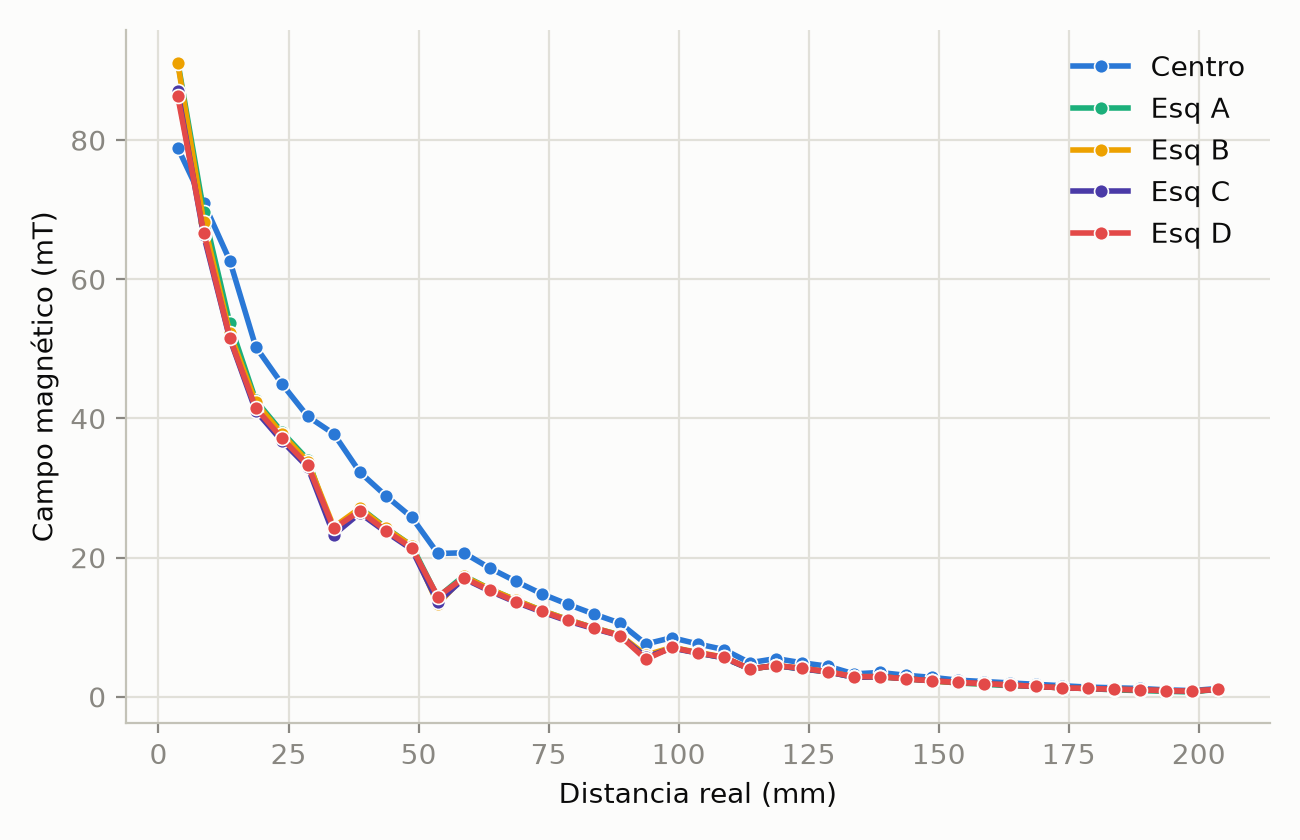
\includegraphics[width=0.85\linewidth]{datos/img/ceramica_n_perfil.png}
    \caption{Caracterización del campo magnético del imán de cerámica, polo norte, en función de la distancia a su cara. Se muestran las mediciones tomadas en el centro y en las cuatro esquinas de la cara del imán.}
    \label{fig:ceramica_n_perfil}
\end{figure}

Un comportamiento equivalente se observó para el imán de cerámica, polo sur (Figura~\ref{fig:ceramica_s_perfil}), donde nuevamente el centro presenta los valores más elevados y las cuatro esquinas se agrupan entre sí, con una caída marcada del campo dentro de los primeros 50~mm.

\begin{figure}[H]
    \centering
    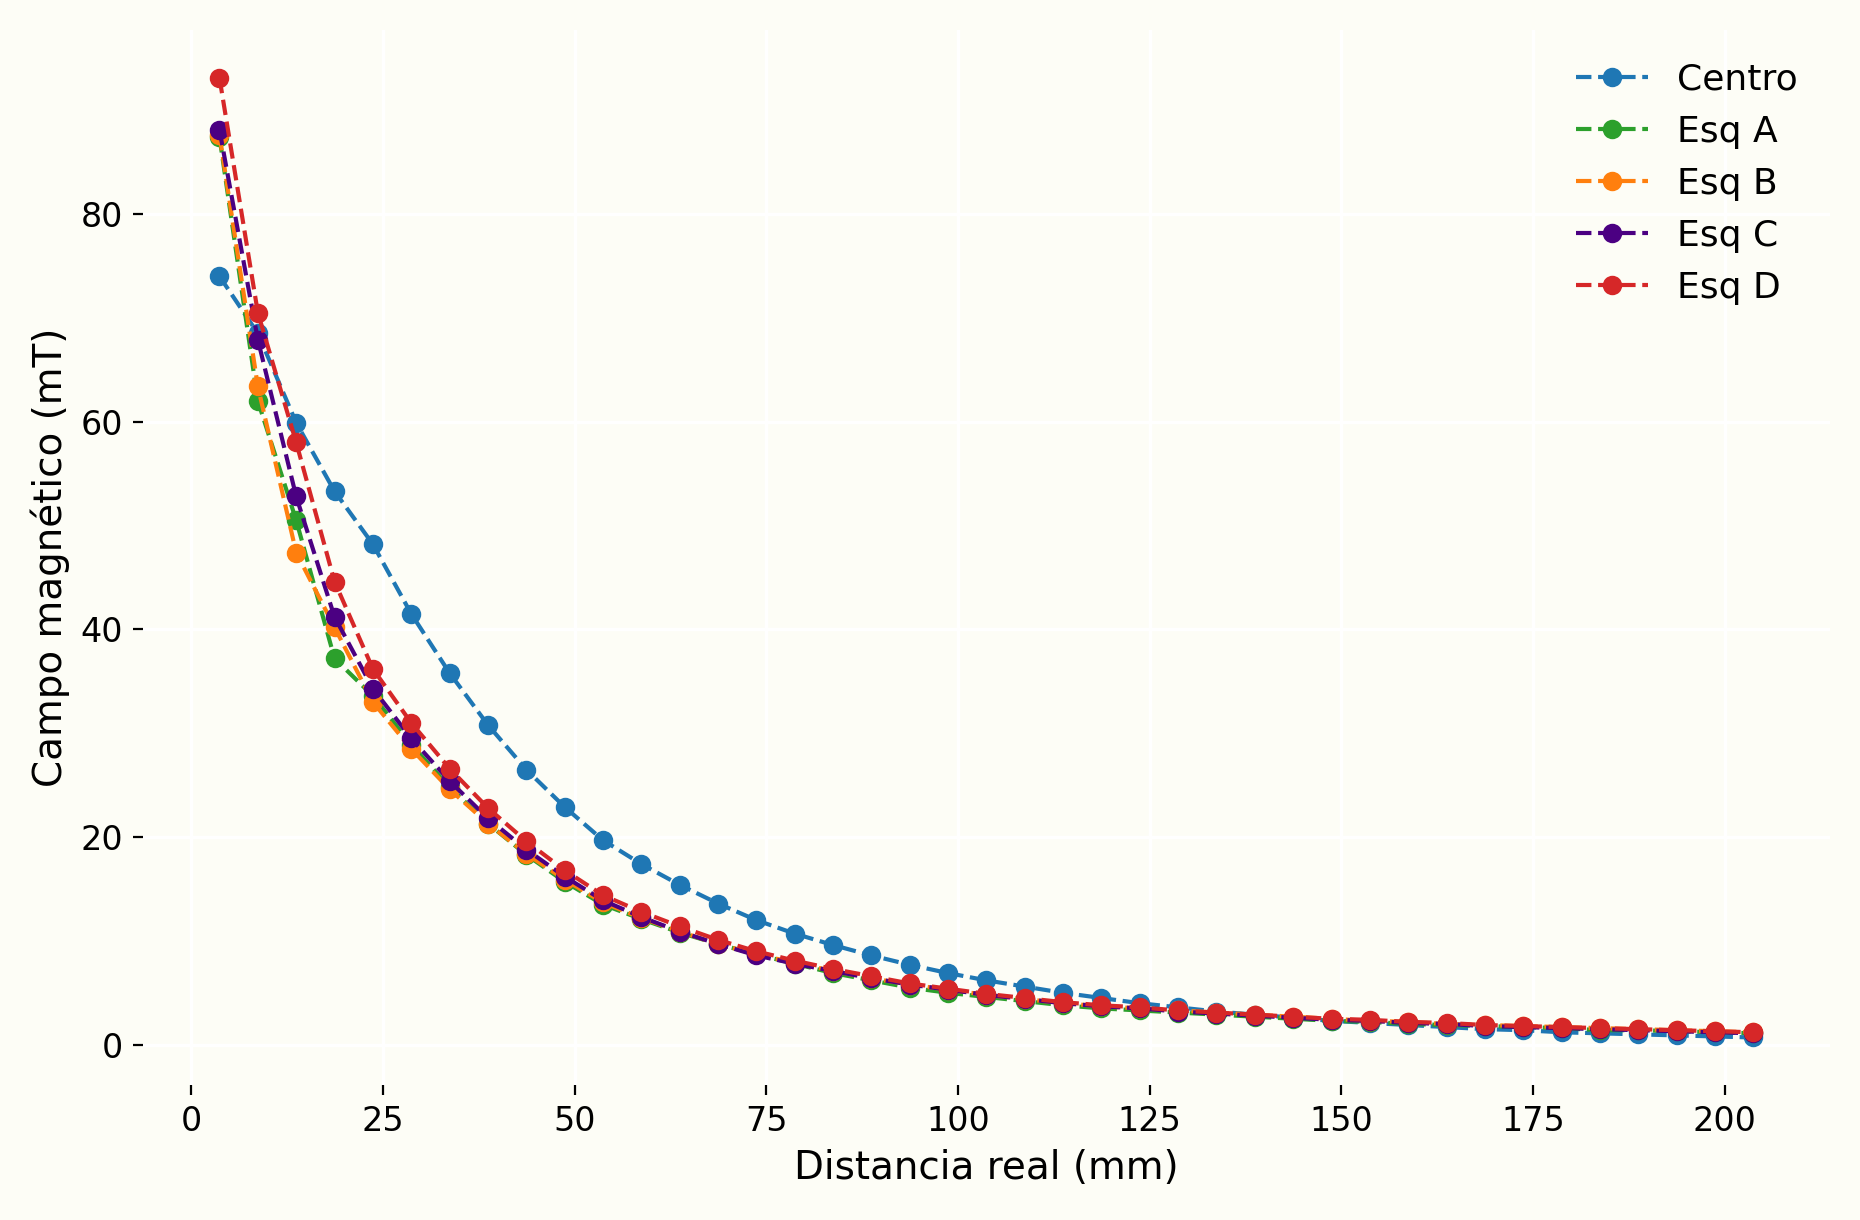
\includegraphics[width=0.85\linewidth]{datos/img/ceramica_s_perfil.png}
    \caption{Caracterización del campo magnético del imán de cerámica, polo sur, en función de la distancia a su cara. Se muestran las mediciones tomadas en el centro y en las cuatro esquinas de la cara del imán.}
    \label{fig:ceramica_s_perfil}
\end{figure}

El imán de neodimio, polo norte, presentó un campo considerablemente más intenso que los imanes de cerámica, alcanzando cerca de 295~mT en el centro a la mínima distancia medida (Figura~\ref{fig:neodimio_n_perfil}). A diferencia de los imanes de cerámica, las mediciones en las esquinas no decrecen monótonamente desde el primer punto, sino que muestran un máximo local a pocos milímetros de la cara antes de decaer, lo cual es consistente con la geometría y distribución de flujo característica de los imanes de neodimio de mayor intensidad.

\begin{figure}[H]
    \centering
    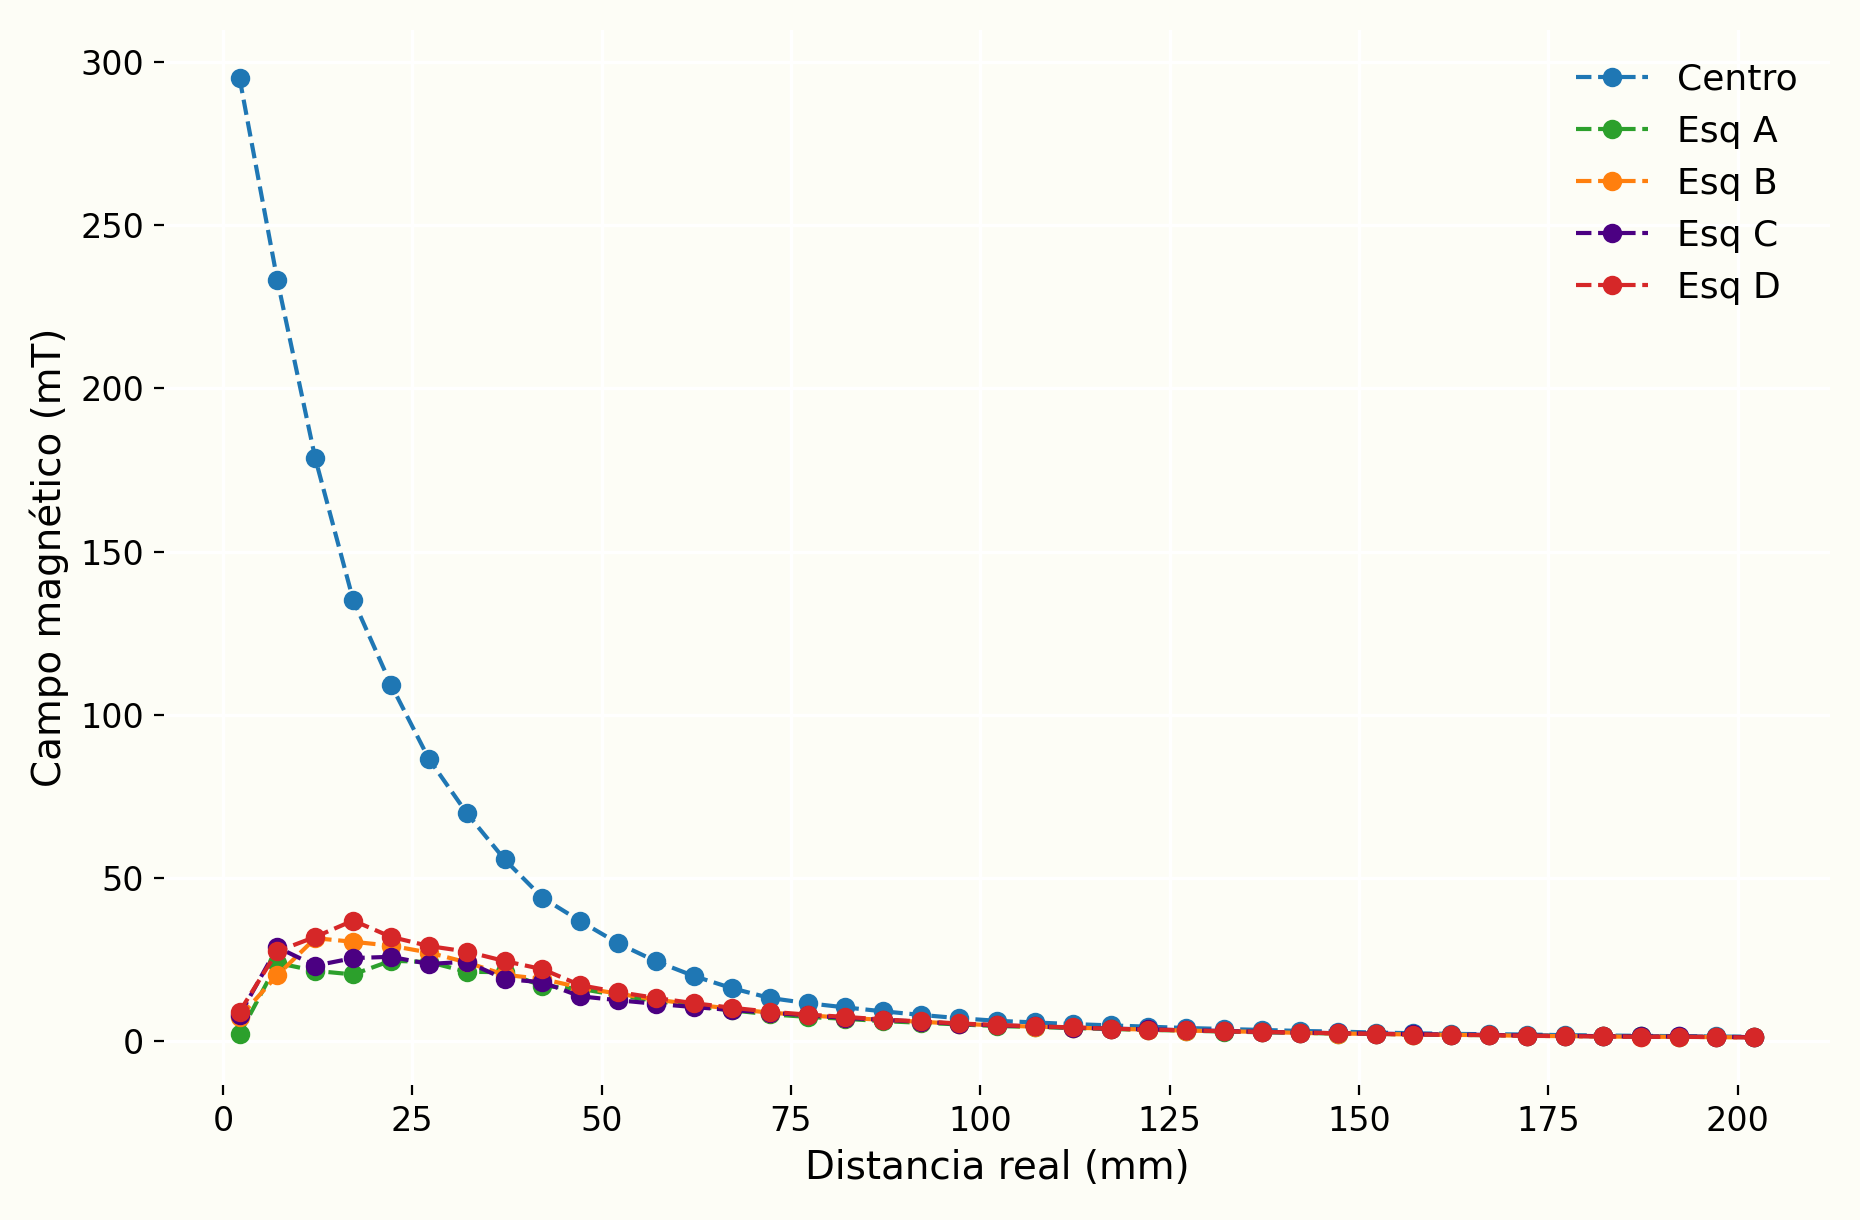
\includegraphics[width=0.85\linewidth]{datos/img/neodimio_n_perfil.png}
    \caption{Caracterización del campo magnético del imán de neodimio, polo norte, en función de la distancia a su cara. Se muestran las mediciones tomadas en el centro y en las cuatro esquinas de la cara del imán.}
    \label{fig:neodimio_n_perfil}
\end{figure}

\subsection{Montaje experimental}

\subsubsection{Diseño de la torre y semilleros}

Se diseñó una estructura experimental compuesta por una torre y un conjunto de semilleros destinada a alojar las semillas durante la etapa de exposición magnética. El objetivo principal de este sistema fue asegurar una disposición geométrica reproducible de las muestras, permitiendo ubicar las semillas en posiciones controladas dentro del montaje experimental.

Durante el diseño se buscó que las piezas cumplieran simultáneamente varios requisitos: contener adecuadamente las semillas, facilitar su manipulación antes y después de la germinación, mantener una disposición estable durante el tratamiento y resultar compatibles con fabricación mediante impresión 3D. Asimismo, se procuró que la geometría del sistema permitiera trabajar de forma ordenada con distintos niveles o posiciones experimentales.

El modelado de la geometría se realizó principalmente en \textit{Tinkercad}, herramienta utilizada para desarrollar la estructura general de la torre y los semilleros. En algunos casos particulares, especialmente cuando se requirieron modificaciones paramétricas o ajustes más sistemáticos, se empleó también \textit{build123d}.

A lo largo del desarrollo fue necesario realizar ajustes sucesivos sobre las dimensiones y el diseño de las piezas, con el fin de mejorar aspectos de calce, estabilidad mecánica y facilidad de uso. Una vez obtenidas versiones satisfactorias, las piezas fueron fabricadas mediante impresión 3D e incorporadas al sistema experimental.

La Figura~\ref{fig:torre_semilleros} muestra, lado a lado, el diseño digital y la pieza ya impresa. Los archivos de diseño y desarrollo asociados se encuentran documentados en el repositorio del proyecto.

\begin{figure}[H]
    \centering
    \begin{subfigure}[b]{0.45\linewidth}
        \centering
        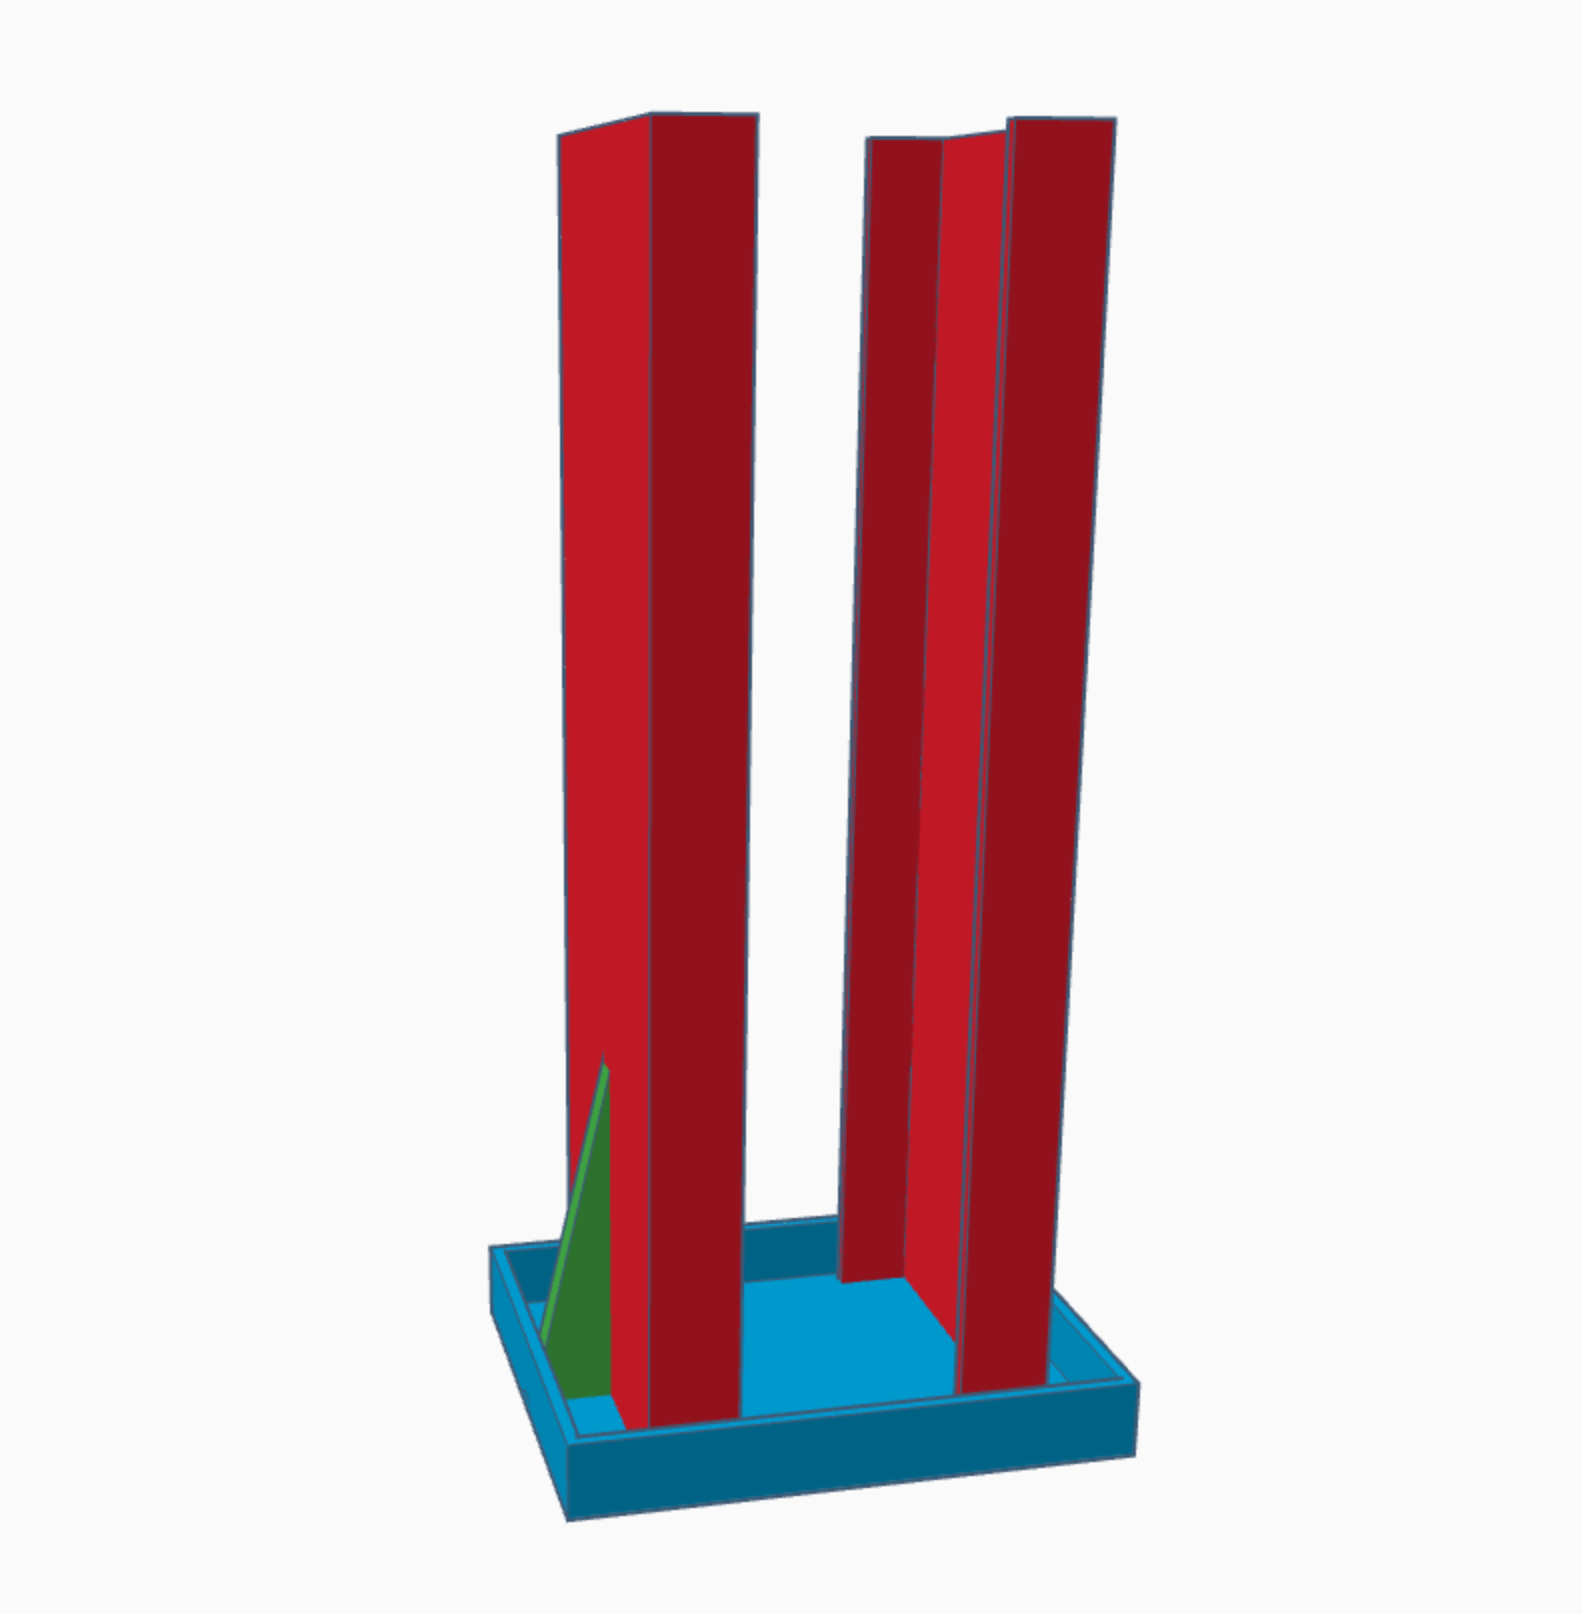
\includegraphics[width=\linewidth]{secciones//images/torre3D.png}
        \caption{Diseño 3D}
    \end{subfigure}
    \hfill
    \begin{subfigure}[b]{0.28\linewidth}
        \centering
        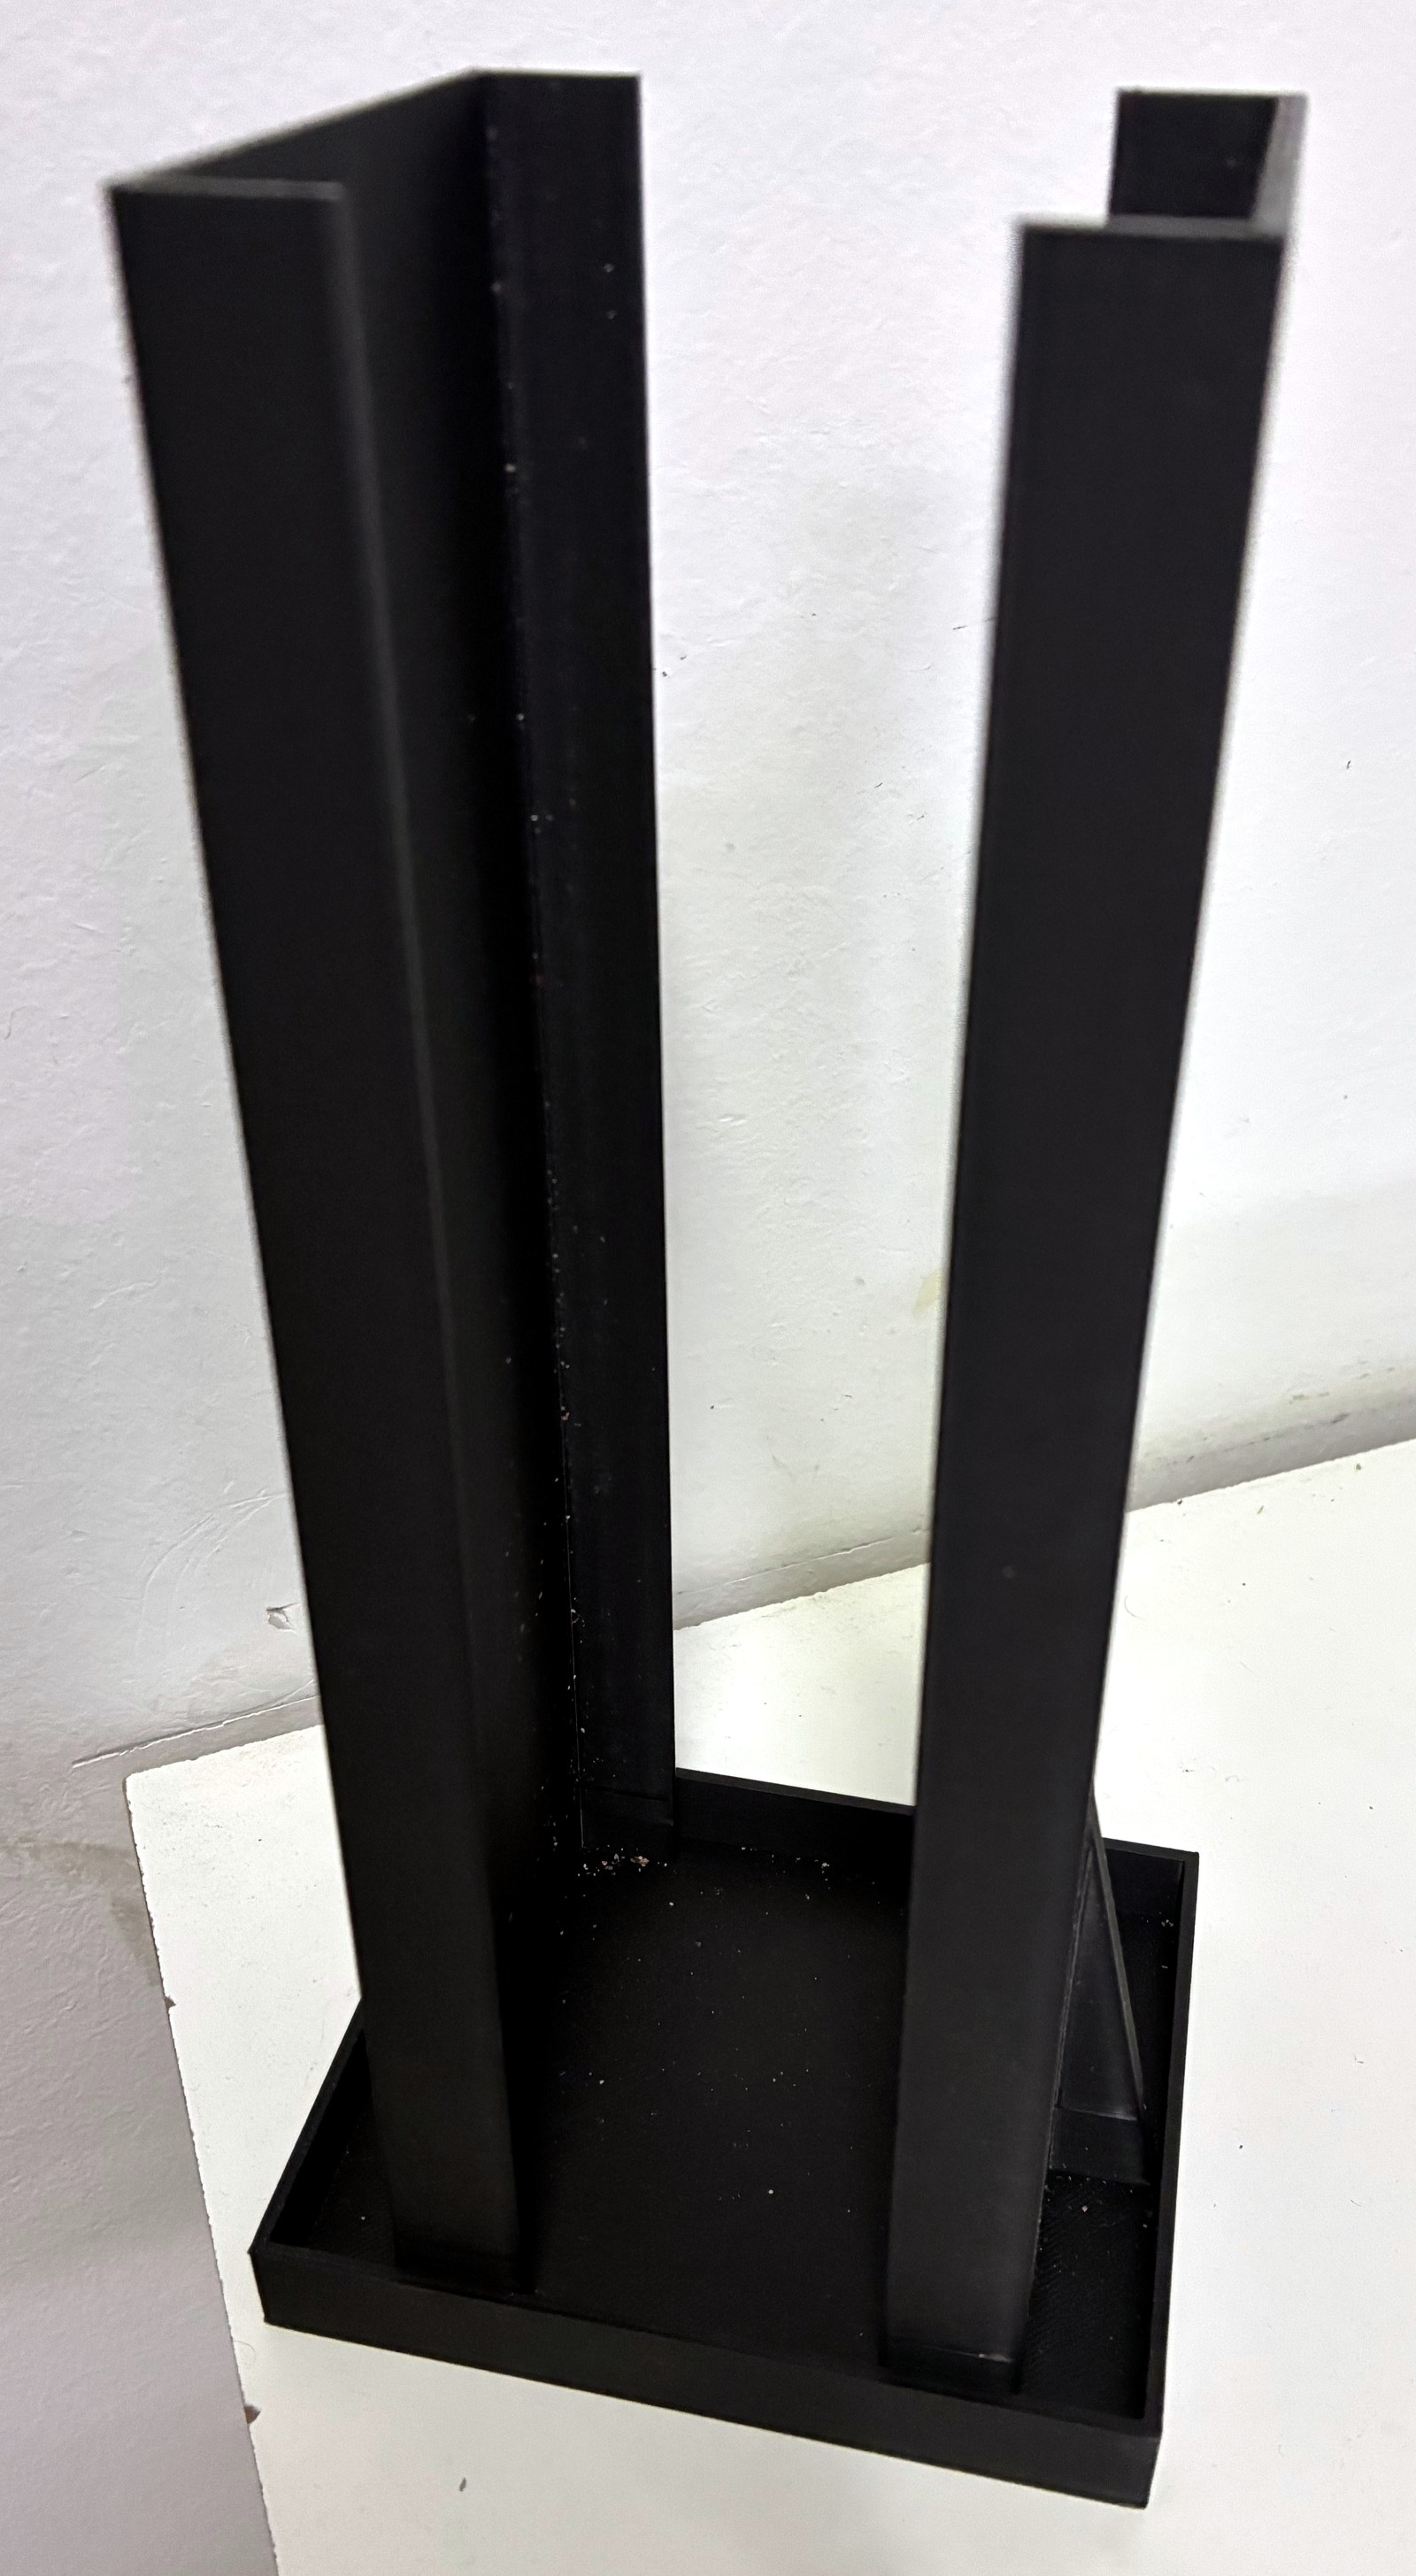
\includegraphics[width=\linewidth]{datos/img/torre_foto.jpg}
        \caption{Pieza impresa}
    \end{subfigure}
    \caption{Torre utilizada para alojar los cajones durante el tratamiento magnético: diseño realizado en \textit{Tinkercad} y pieza final fabricada mediante impresión 3D.}
    \label{fig:torre_semilleros}
\end{figure}

\subsubsection{Cajón portasemillas}

Como parte de este sistema, se diseñó un cajón destinado a contener las semillas durante el tratamiento. En su diseño se buscó que permitiera una disposición ordenada de las muestras, facilitara su manipulación y resultara compatible con el resto de la estructura experimental. Asimismo, se procuró que sus dimensiones fueran adecuadas para el alojamiento de las semillas y para su fabricación mediante impresión 3D.

El modelado de estas piezas se realizó principalmente en \textit{Tinkercad}, complementado en algunos casos con \textit{build123d} para ajustes paramétricos. Las versiones finales fueron fabricadas mediante impresión 3D. En la Figura~\ref{fig:cajon_semillas} se muestra, lado a lado, el diseño y la pieza física utilizada.

\begin{figure}[H]
    \centering
    \begin{subfigure}[b]{0.45\linewidth}
        \centering
        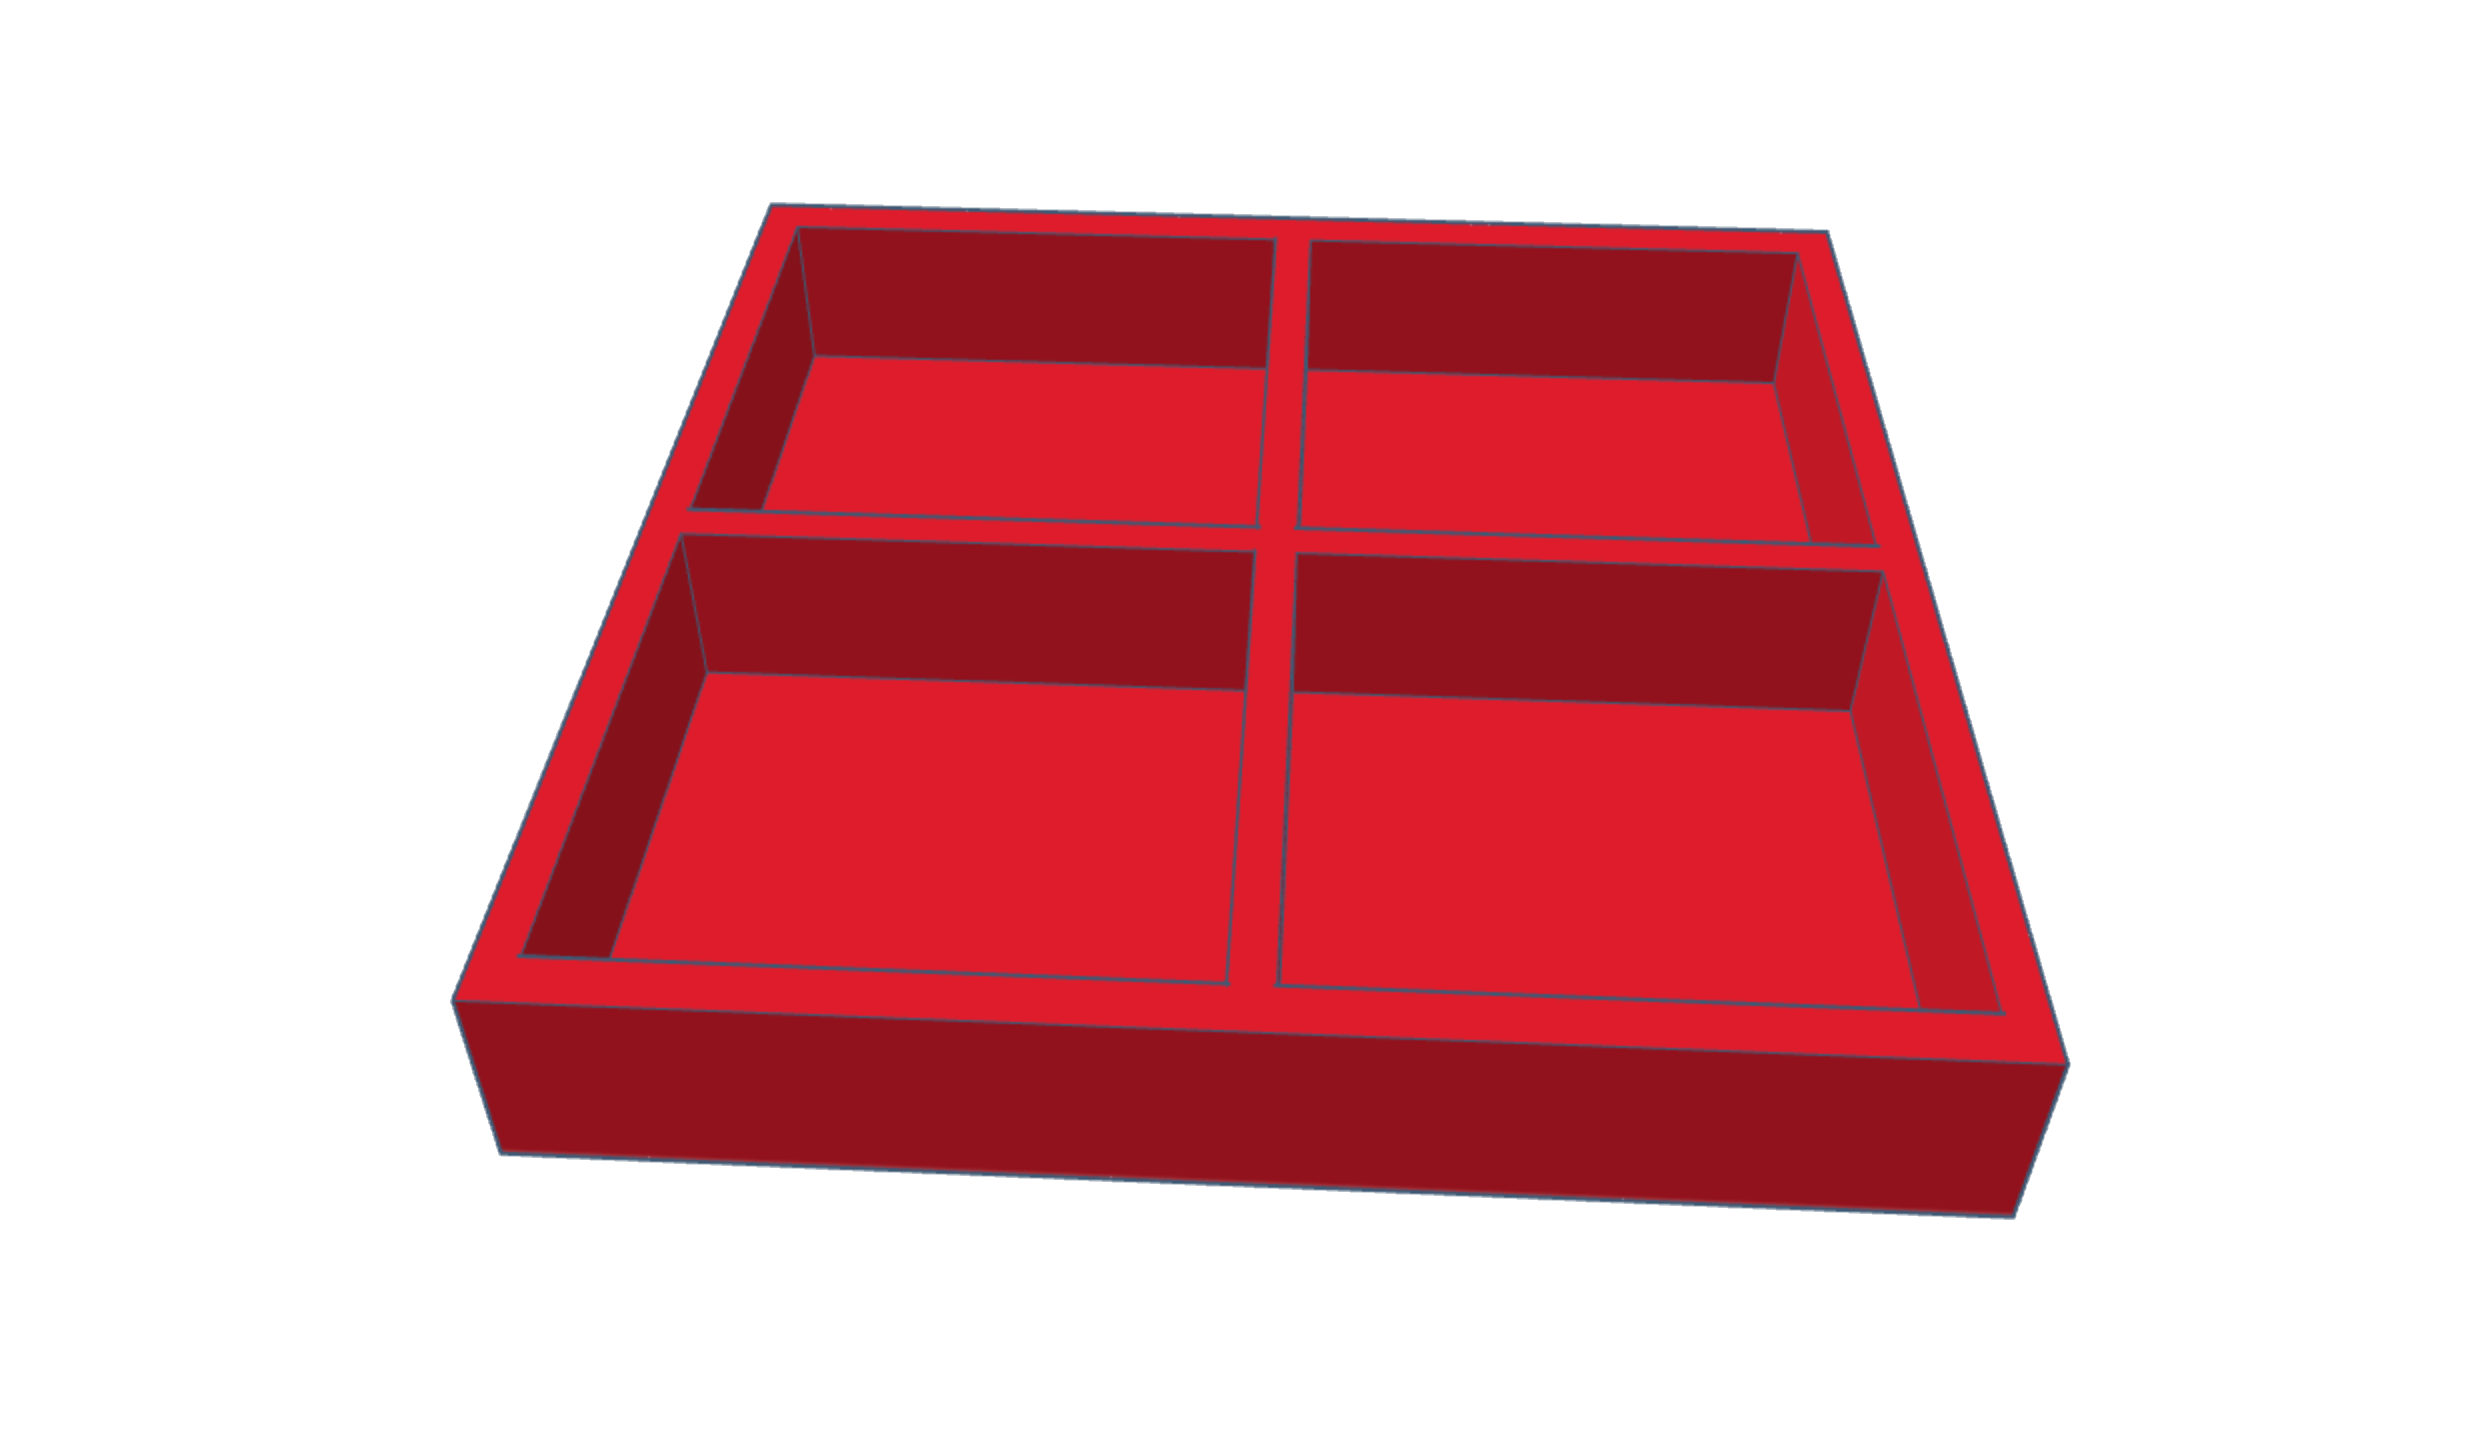
\includegraphics[width=\linewidth]{secciones//images/cajon3D.png}
        \caption{Diseño 3D}
    \end{subfigure}
    \hfill
    \begin{subfigure}[b]{0.45\linewidth}
        \centering
        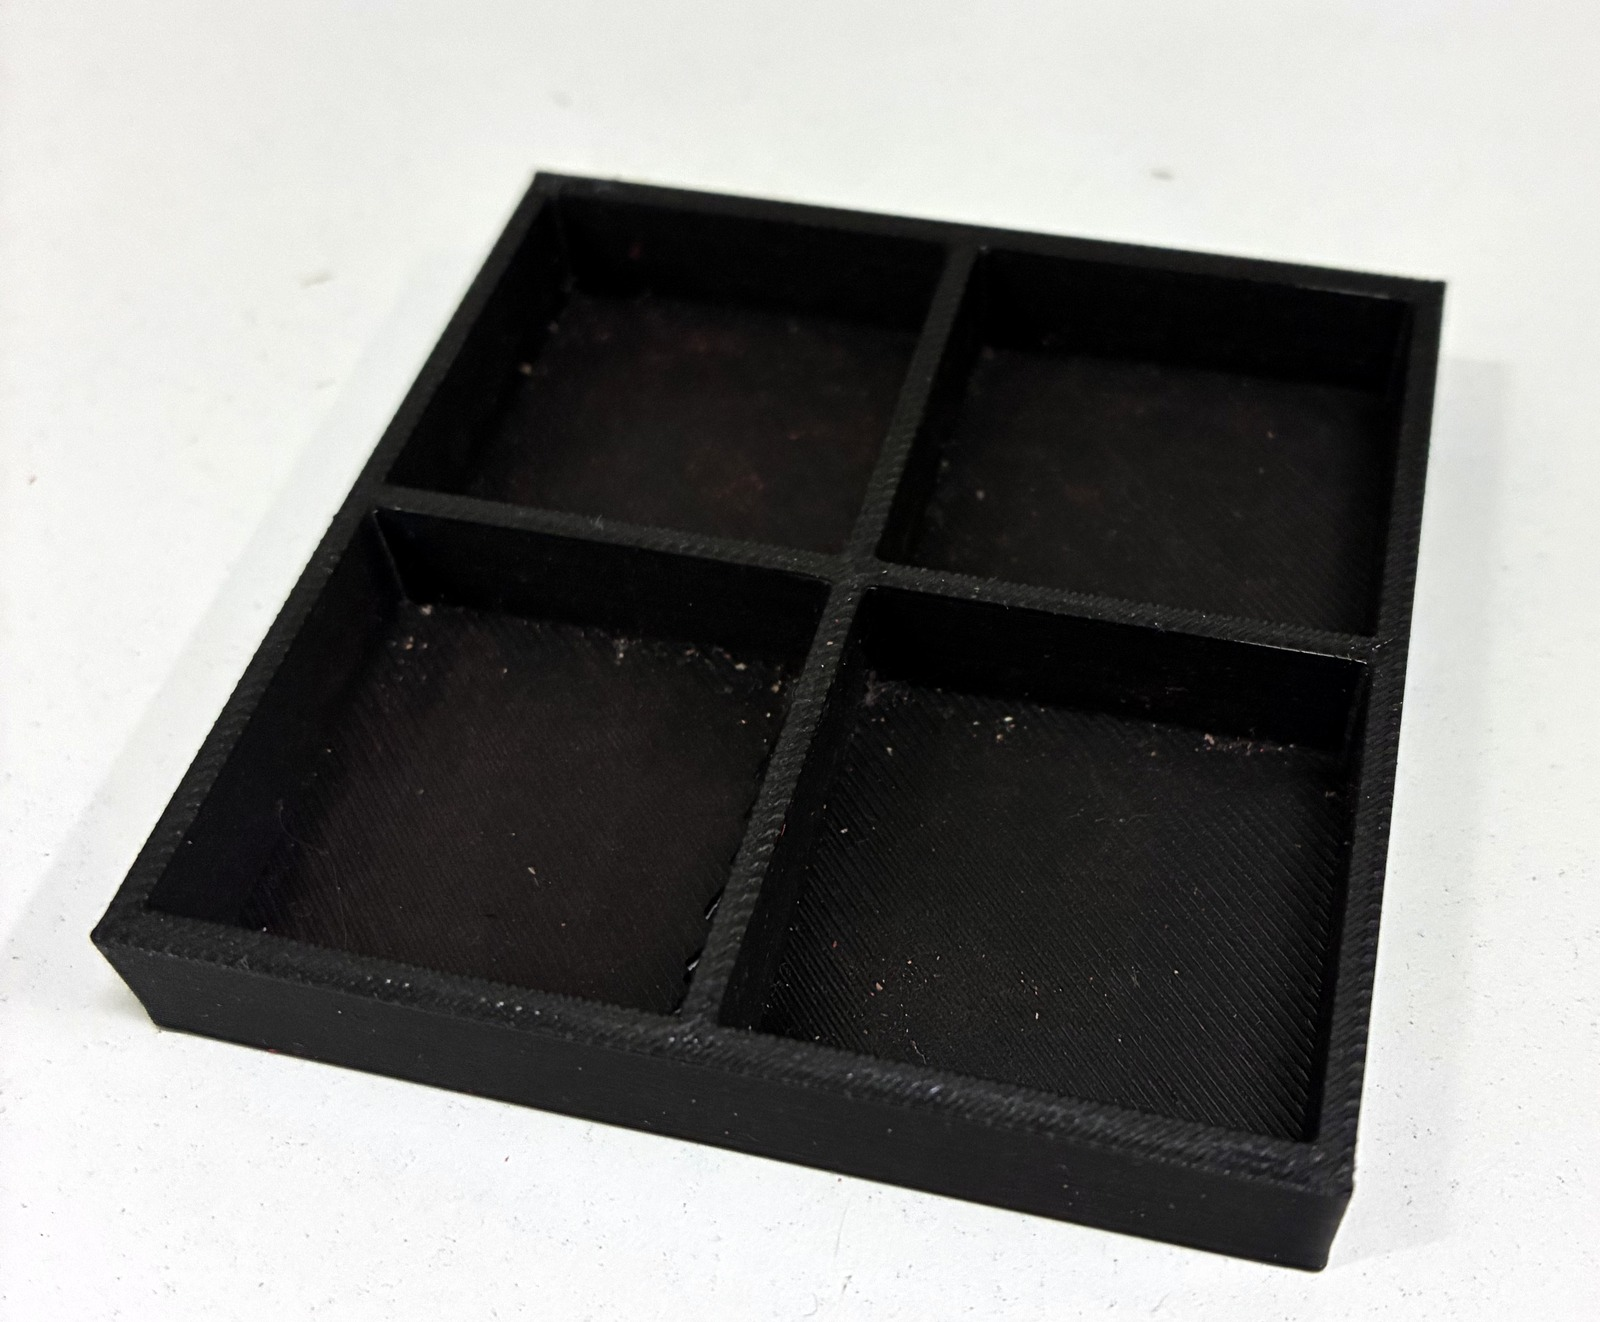
\includegraphics[width=\linewidth]{datos/img/cajon_foto.jpg}
        \caption{Pieza impresa}
    \end{subfigure}
    \caption{Cajón portasemillas con cuatro compartimentos para el alojamiento de semillas: diseño y pieza fabricada mediante impresión 3D.}
    \label{fig:cajon_semillas}
\end{figure}

\subsubsection{Piezas auxiliares para manipulación experimental}

Además de la estructura principal de tratamiento, se diseñaron piezas auxiliares destinadas a facilitar distintas etapas del trabajo experimental. Entre ellas se incluyó una cubierta parcial para cajones y una cuchara medidora para la dosificación de semillas.

\subsubsection{Dispositivo de dosificación de semillas}

Con el fin de evitar el conteo manual repetido de 20 semillas por muestra, se diseñó una cuchara medidora orientada a dosificar aproximadamente esa cantidad con la menor variabilidad posible. Dado que el volumen ocupado por las semillas depende de su tamaño y disposición, se optó por un diseño paramétrico utilizando \textit{build123d}, lo que permitió modificar de manera sistemática las dimensiones de la pieza.

A partir de un diseño inicial, se generaron variantes con cambios de tamaño del orden de $\pm 5\%$, con el objetivo de evaluar cuál de ellas se ajustaba mejor a una carga cercana a 20 semillas de maíz por uso. Las distintas versiones fueron fabricadas mediante impresión 3D y comparadas experimentalmente, seleccionándose finalmente aquella que mostró el mejor ajuste al valor buscado y una menor variabilidad entre repeticiones. La caracterización de la cuchara seleccionada, realizada a partir de 108 mediciones, mostró una media de 17,44 semillas por carga, una mediana de 17,00 semillas y una desviación estándar de 2,08 semillas. Se agradece a Lucía Guerreiro por la obtención y provisión de estos datos.

La Figura~\ref{fig:cuchara3D} muestra, lado a lado, el diseño digital y la cuchara medidora ya impresa. Los archivos de diseño correspondientes se encuentran documentados en el repositorio del proyecto.

\begin{figure}[H]
    \centering
    \begin{subfigure}[b]{0.45\linewidth}
        \centering
        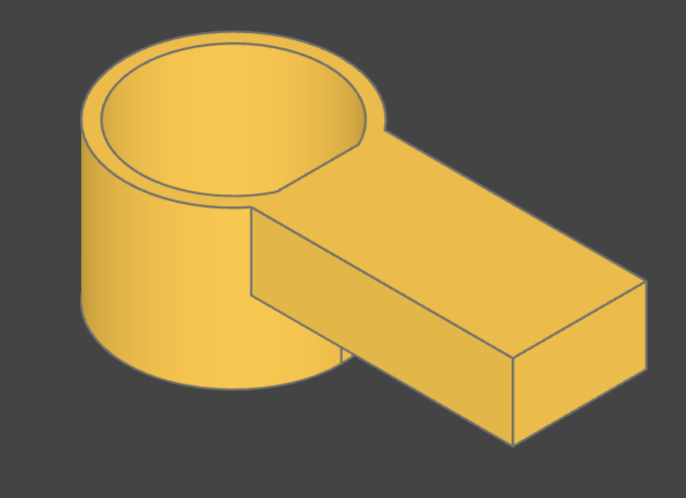
\includegraphics[width=\linewidth]{secciones//images/cuchara3D.png}
        \caption{Diseño 3D}
    \end{subfigure}
    \hfill
    \begin{subfigure}[b]{0.45\linewidth}
        \centering
        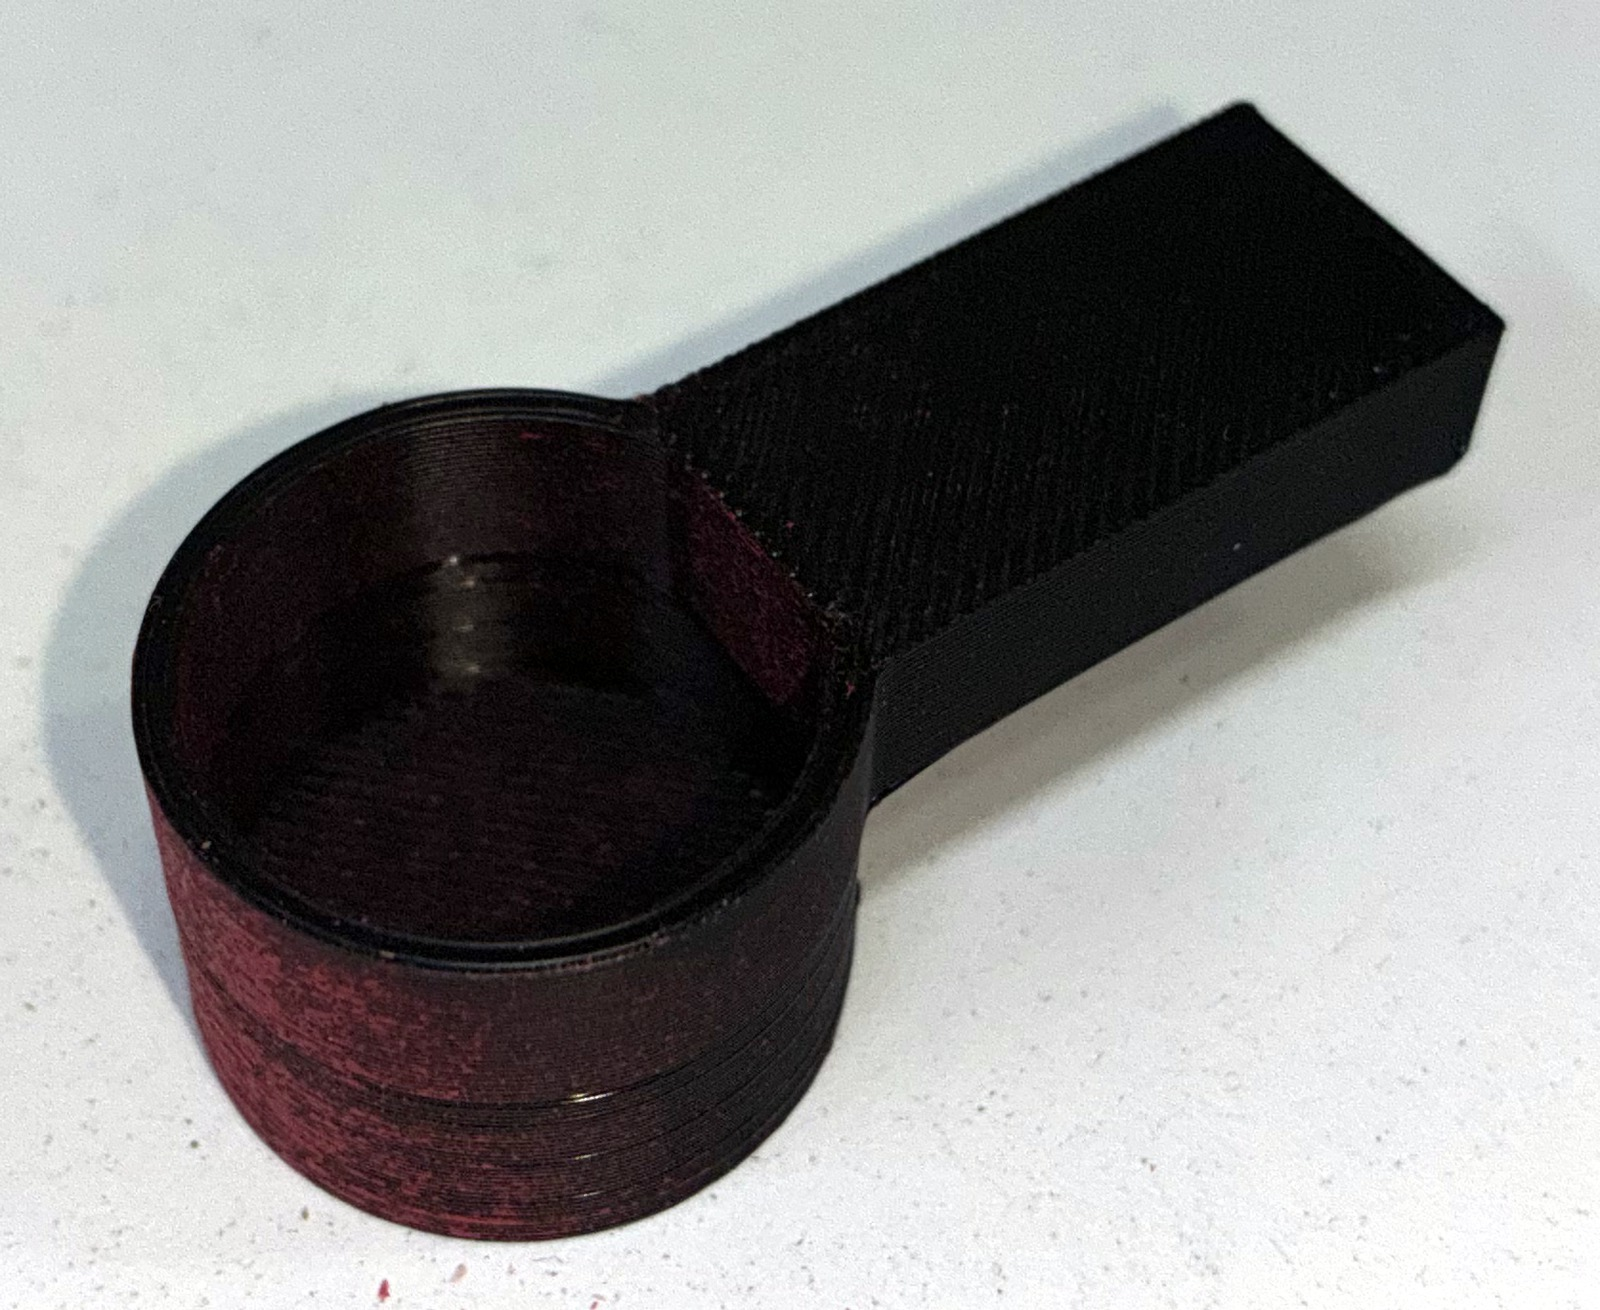
\includegraphics[width=\linewidth]{datos/img/cuchara_foto.jpg}
        \caption{Pieza impresa}
    \end{subfigure}
    \caption{Cuchara medidora desarrollada para dosificar aproximadamente 20 semillas de maíz: diseño y pieza fabricada mediante impresión 3D.}
    \label{fig:cuchara3D}
\end{figure}

\begin{figure}[H]
    \centering
    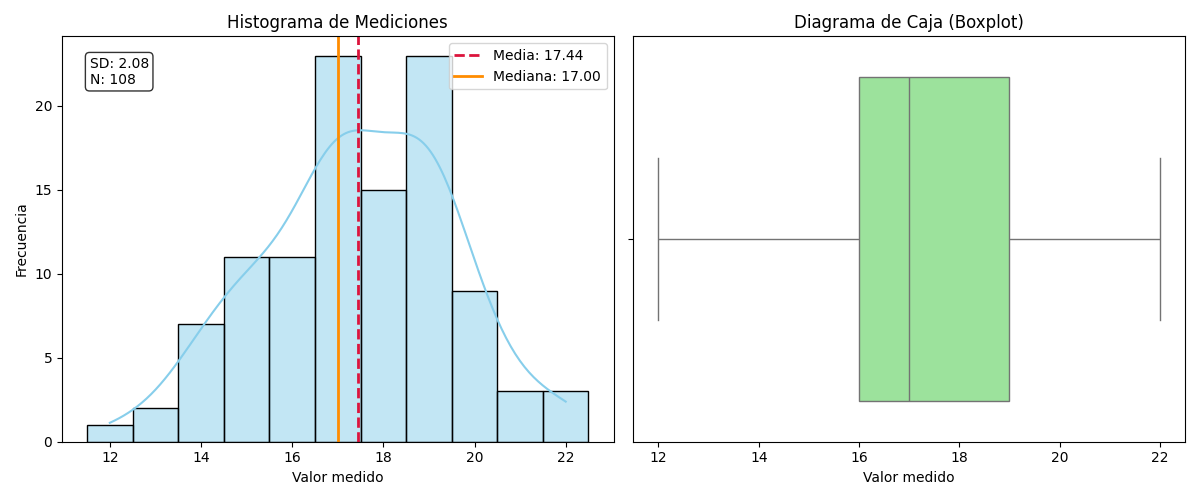
\includegraphics[width=\linewidth]{secciones//images/CaracterizacionCucharaPlots.png}
    \caption{Caracterización experimental de la cuchara medidora seleccionada. Se muestra la distribución de las mediciones de cantidad de semillas por carga y el diagrama de caja correspondiente.}
    \label{fig:caracterizacion_cuchara}
\end{figure}

\subsubsection{Construcción del photobox}

Para la adquisición de imágenes de semillas germinadas se construyó un \textit{photobox}, consistente en una caja con fondo negro e iluminación LED. Este dispositivo fue diseñado con el propósito de mejorar el contraste de las imágenes y estandarizar las condiciones de captura, reduciendo la variabilidad asociada a la iluminación y al fondo durante la toma fotográfica.

La utilización de este sistema permitió obtener imágenes en condiciones más homogéneas, facilitando posteriormente el procesamiento automático de las radículas mediante software.

\subsection{Procedimiento experimental}

Los experimentos se llevaron a cabo empleando el sistema de torre, semilleros y cajones diseñado para este trabajo. Las semillas fueron distribuidas en bandejas o recipientes identificados de forma individual, de manera de conservar la trazabilidad de cada unidad experimental durante las distintas etapas del protocolo.

La organización espacial de las muestras dentro del sistema experimental fue asistida mediante una asignación controlada de posiciones, con el objetivo de ordenar la disposición de las semillas dentro del montaje y disminuir posibles sesgos asociados a la ubicación de las muestras. Asimismo, se procuró mantener condiciones de trabajo reproducibles durante las etapas de preparación, tratamiento, germinación y registro.

Luego del tratamiento y de la etapa de germinación, las muestras fueron fotografiadas utilizando el \textit{photobox} construido para este trabajo. Dichas imágenes constituyeron la base para el procesamiento posterior de las radículas mediante herramientas computacionales específicas.

\subsection{Registro de datos}

Con el fin de asegurar un registro sistemático de la información experimental, se generó para cada ensayo una estructura de directorios y archivos en la que se almacenaron tanto los datos descriptivos del experimento como los resultados obtenidos durante las distintas etapas del trabajo.

En particular, se registró la identificación de cada bandeja, su posición dentro del montaje experimental, la asignación correspondiente dentro del esquema de tratamiento y metadatos asociados al experimento, tales como el imán utilizado y el polo enfrentado a las semillas. Asimismo, se incorporó la posibilidad de registrar pesos iniciales y finales de cada unidad experimental, facilitando una organización estructurada de la información.

Las fotografías adquiridas durante la etapa de germinación también fueron almacenadas de manera ordenada dentro de la estructura del proyecto, de modo de conservar la trazabilidad entre las imágenes, las bandejas y los resultados del análisis posterior.

\subsection{Herramientas computacionales desarrolladas}

Además del desarrollo del montaje físico, se implementaron herramientas computacionales orientadas a asistir la organización del experimento, el registro de datos y el procesamiento automático de imágenes. Estas herramientas constituyeron un soporte metodológico para mejorar la trazabilidad, reproducibilidad y eficiencia del flujo de trabajo experimental.

\subsubsection{Asignador de bandejas}

Como parte de las herramientas computacionales desarrolladas para este trabajo, se implementó un programa en Python destinado a la asignación y gestión de las bandejas experimentales. Su propósito fue asistir la organización de cada ensayo mediante la creación automática de la estructura de archivos asociada al experimento, la generación del archivo \texttt{trays.csv} y la asignación aleatoria de los tratamientos a las posiciones físicas disponibles en el arreglo experimental.

El programa permitió definir e identificar cada bandeja de manera unívoca, asociándola al experimento correspondiente y a su posición dentro del montaje. Además, incorporó el registro de metadatos experimentales, tales como el imán utilizado y el polo enfrentado a las semillas. De este modo, se facilitó la trazabilidad de cada unidad experimental y la conservación ordenada de la información relevante para el posterior análisis de datos.

Adicionalmente, la herramienta incluyó una interfaz para la carga y actualización de los pesos iniciales y finales de las bandejas, con sugerencias automáticas de la siguiente posición a completar. Esta funcionalidad permitió agilizar la carga secuencial de datos y reducir la probabilidad de errores manuales durante el registro. En conjunto, el asignador de bandejas constituyó una herramienta auxiliar para estandarizar la organización del experimento, mejorar la reproducibilidad del procedimiento y favorecer la consistencia del registro experimental.

En la Figura~\ref{fig:asignador-bandejas} se muestra una captura de la interfaz gráfica desarrollada para esta herramienta.

\begin{figure}[H]
    \centering
    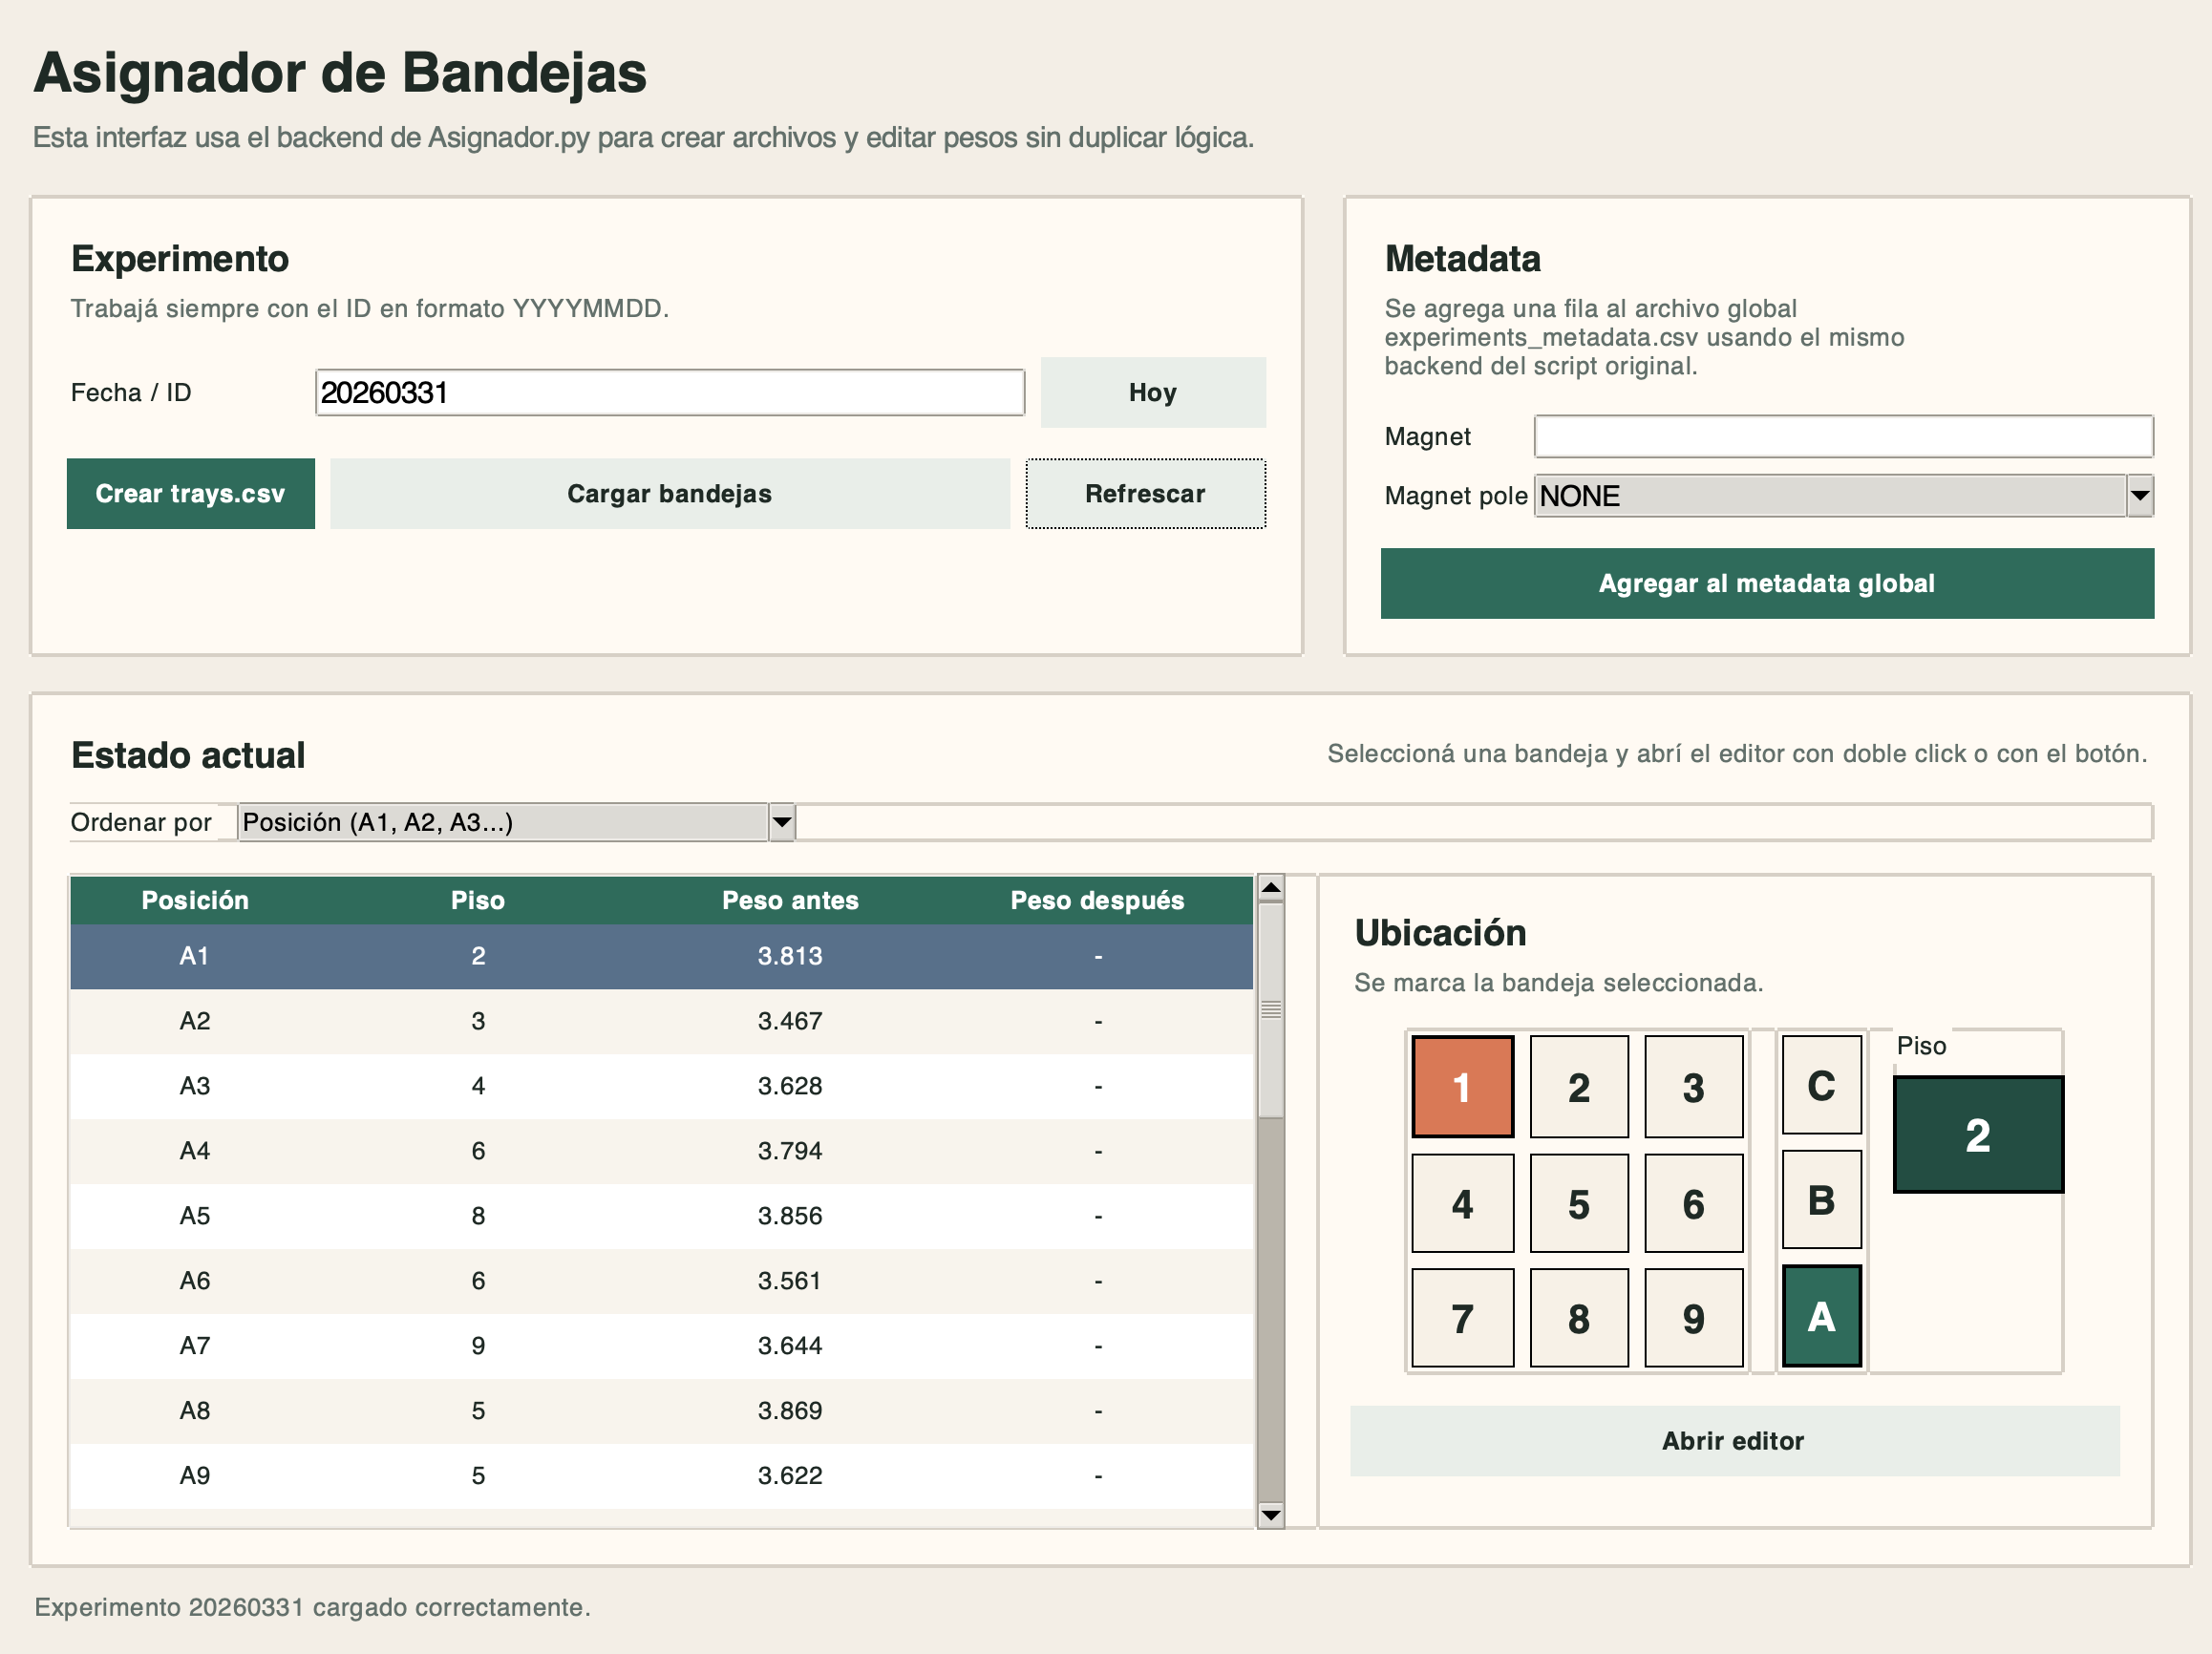
\includegraphics[width=0.75\linewidth]{secciones//images/asignadorGUI.png}
    \caption{Interfaz gráfica del programa desarrollado para la asignación y gestión de bandejas experimentales.}
    \label{fig:asignador-bandejas}
\end{figure}

\subsection{Procesamiento y análisis de datos}

Una vez adquiridas las imágenes de las semillas germinadas, se realizó un procesamiento automático orientado a extraer parámetros cuantitativos asociados al crecimiento de las radículas. Para ello se desarrolló una herramienta específica que permitió identificar estructuras de interés en las imágenes, medir sus longitudes y almacenar los resultados obtenidos de manera organizada para su posterior análisis.

\subsubsection{Software de detección y medición de radículas}

Se desarrolló una herramienta de software para el procesamiento automático de imágenes de semillas germinadas, con el objetivo de estimar la longitud de las radículas a partir de fotografías adquiridas mediante el \textit{photobox}. El programa permite identificar las radículas presentes en cada imagen, calcular sus longitudes individuales y obtener medidas agregadas, como la longitud media de radícula por muestra.

La implementación de esta herramienta tuvo como finalidad reducir la intervención manual en la etapa de medición, mejorar la reproducibilidad del procesamiento y facilitar el almacenamiento sistemático de los resultados experimentales. Los datos generados por el software fueron utilizados posteriormente en la etapa de análisis.

La Figura~\ref{fig:software_radiculas} presenta una captura de pantalla de la interfaz o entorno de uso del software desarrollado. El código correspondiente se encuentra disponible en el repositorio del proyecto.

\begin{figure}[H]
    \centering
    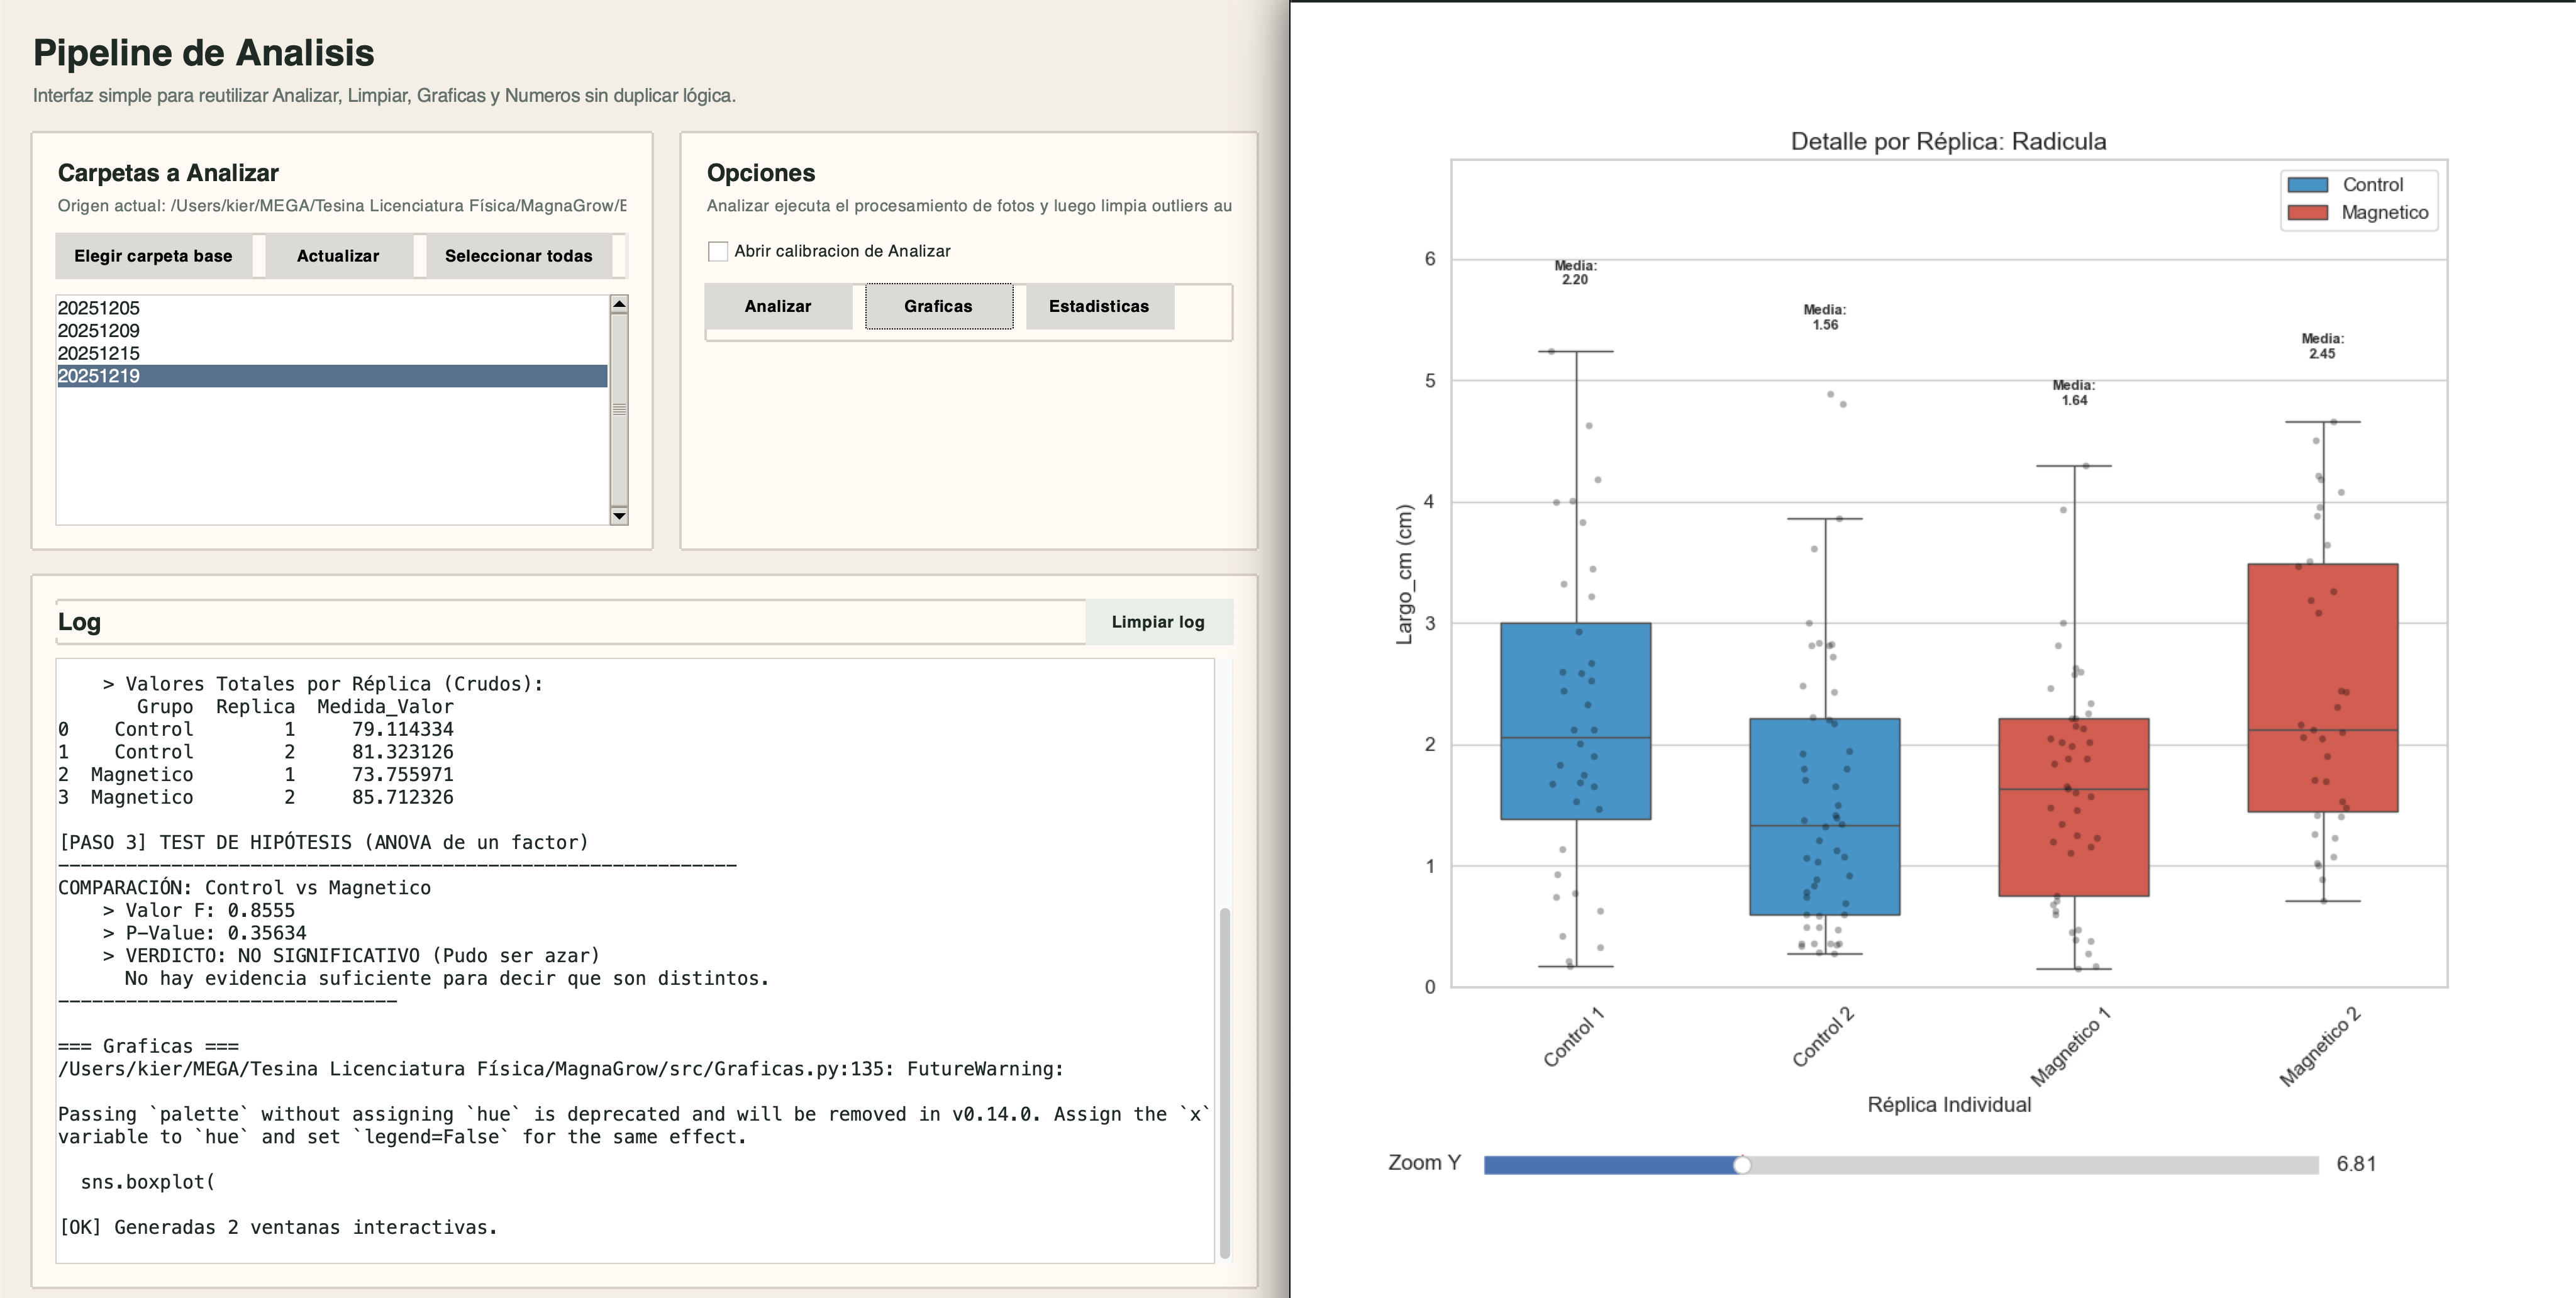
\includegraphics[width=1\linewidth]{secciones//images/pipelineGUI.png}
    \caption{Interfaz del software desarrollado para el procesamiento de imágenes y la obtención de parámetros cuantitativos a partir de fotografías de semillas germinadas.}
    \label{fig:software_radiculas}
\end{figure}

\subsection{Experimentos control negativo}

Con el objetivo de caracterizar la variabilidad basal del sistema experimental y establecer una línea de referencia para la comparación con los tratamientos magnéticos, se realizaron tres experimentos control independientes en los que las semillas no estuvieron expuestas a ningún campo magnético. Estos experimentos se llevaron a cabo en las fechas 04/04/2026, 28/04/2026 y 07/05/2026.

Cada experimento control consistió en 27 bandejas experimentales, distribuidas en 3 pisos (A, B, C) y 9 posiciones, siguiendo la misma disposición geométrica y el mismo protocolo de germinación, registro fotográfico y procesamiento de imágenes que los experimentos con tratamiento. No se colocaron imanes en ninguna de las bandejas durante la etapa de exposición.

El diseño repetido en el tiempo permitió evaluar la reproducibilidad del protocolo y cuantificar la variabilidad interexperimento atribuible a factores no controlados, como fluctuaciones ambientales o diferencias entre lotes de semillas. Asimismo, el diseño espacial (piso y posición) posibilitó la detección de posibles sesgos sistemáticos dentro del montaje experimental, información relevante para la interpretación de los resultados de los experimentos con tratamiento.

\section{Resultados}

\subsection{Controles negativos}

Se realizaron tres experimentos de 72\,h los días 20260404, 20260428 y 20260507, para un total de \(n = 81\) bandejas (27 por día). La variable principal de análisis fue el \textbf{cambio porcentual de peso} (\emph{pct\_change} en el código de análisis), definido como el aumento de masa respecto al peso inicial de las semillas en cada bandeja. Como verificación de robustez, los principales análisis se repitieron con dos variables de crecimiento alternativas: el \textbf{cambio absoluto de peso} (\emph{raw\_delta\_weight}), definido como la diferencia entre el peso final e inicial en gramos, y el \textbf{logaritmo de la razón de pesos} (\emph{raw\_log\_ratio}), definido como el logaritmo natural del cociente entre el peso final y el inicial. Estas tres variables cuantifican el mismo fenómeno de crecimiento con distintas propiedades estadísticas; su coincidencia en dirección y significancia refuerza que los efectos reportados no dependen de la métrica elegida.

\subsubsection{Supuestos estadísticos}

Se evaluó la normalidad de los residuos mediante el test de Shapiro-Wilk y la homogeneidad de varianzas mediante el test de Brown-Forsythe. Para el cambio porcentual de peso, los residuos resultaron normales (\(p = 0.5773\)) pero las varianzas no resultaron homogéneas entre días (\(p = 0.0302\)). Por lo tanto, los modelos presentados a continuación fueron ajustados por día experimental y utilizan errores robustos HC3 para compensar la heterogeneidad de varianzas.

\subsubsection{Calidad del armado (pesos iniciales)}

Para descartar un posible sesgo de selección al momento de armar las bandejas, se analizó si las semillas iniciales tenían masas diferentes entre pisos. El resultado no fue significativo (\(p = 0.4926\)), lo que indica que los pisos A, B y C comenzaron con masas de semillas estadísticamente equivalentes. Las diferencias observadas al final del experimento se atribuyen, por lo tanto, a factores ocurridos durante el crecimiento y no a un sesgo inicial.

\subsubsection{Efecto del piso (A, B, C)}

La Figura~\ref{fig:ctrl_pct_change_floor} muestra el crecimiento relativo promedio para cada piso. La Tabla~\ref{tab:ctrl_floor} presenta las medias y desvíos estándar.

\begin{table}[h]
\centering
\caption{Crecimiento relativo (cambio porcentual de peso) por piso en controles negativos combinados. Los valores se expresan como media \(\pm\) SD entre bandejas dentro de cada grupo (\(n = 27\) por piso).}
\label{tab:ctrl_floor}
\begin{tabular}{lc}
\hline
Piso & Media \(\pm\) SD \\
\hline
A & 0.4455 \(\pm\) 0.0376 \\
B & 0.4261 \(\pm\) 0.0448 \\
C & 0.4094 \(\pm\) 0.0534 \\
\hline
\end{tabular}
\end{table}

Se observaron diferencias significativas entre pisos (\(F_{2,76} = 3.9746\), \(p = 0.0228\)), con un patrón consistente A \(>\) B \(>\) C en crecimiento promedio.

Como verificación de robustez, el mismo análisis se repitió utilizando el cambio absoluto de peso y el logaritmo de la razón de pesos. La Tabla~\ref{tab:ctrl_floor_robustez} presenta las medias y desvíos estándar por piso para ambas variables, junto con los resultados del test de diferencias.

\begin{table}[h]
\centering
\caption{Crecimiento por piso para el cambio absoluto de peso y el logaritmo de la razón de pesos, como verificación de robustez del efecto observado con el cambio porcentual de peso. Los valores se expresan como media \(\pm\) SD entre bandejas dentro de cada grupo (\(n = 27\) por piso).}
\label{tab:ctrl_floor_robustez}
\begin{tabular}{lcccc}
\hline
Variable & Piso A & Piso B & Piso C & \(F_{2,76}\) (\(p\)) \\
\hline
Cambio absoluto de peso & 1.6412 \(\pm\) 0.1463 & 1.5860 \(\pm\) 0.1796 & 1.4892 \(\pm\) 0.1964 & 4.7870 (0.0110) \\
Logaritmo razón de pesos & 0.3681 \(\pm\) 0.0261 & 0.3545 \(\pm\) 0.0314 & 0.3425 \(\pm\) 0.0378 & 4.0686 (0.0210) \\
\hline
\end{tabular}
\end{table}

Ambas variables reproducen el mismo patrón A \(>\) B \(>\) C y alcanzan significancia estadística, confirmando que el efecto de piso no depende de la métrica de crecimiento elegida. Adicionalmente, se verificó el resultado mediante un ANOVA clásico ajustado por día experimental (sin errores robustos), obteniéndose resultados consistentes para las tres variables (Tabla~\ref{tab:ctrl_floor_anova_clasico}).

\begin{table}[h]
\centering
\caption{Verificación del efecto de piso mediante ANOVA clásico ajustado por día experimental.}
\label{tab:ctrl_floor_anova_clasico}
\begin{tabular}{lcc}
\hline
Variable & \(F\) clásico & \(p\) clásico \\
\hline
Cambio absoluto de peso & 5.1563 & 0.00794 \\
Cambio porcentual de peso & 4.2663 & 0.0175 \\
Logaritmo razón de pesos  & 4.3650 & 0.0161 \\
\hline
\end{tabular}
\end{table}

\begin{figure}[H]
    \centering
    \includegraphics[width=0.75\linewidth]{datos/software_data/analysis/negative_control_combined/negative_control_combined_pct_change_floor_barplot.png}
    \caption{Crecimiento relativo (cambio porcentual de peso) por piso en controles negativos combinados. Cada punto corresponde a una bandeja individual, coloreada según el día del experimento.}
    \label{fig:ctrl_pct_change_floor}
\end{figure}

\subsubsection{Efecto de la posición lateral (izquierda, centro, derecha)}

La Figura~\ref{fig:ctrl_pct_change_lcr} muestra el crecimiento según la posición lateral. La Tabla~\ref{tab:ctrl_lcr} presenta los valores numéricos.

\begin{table}[h]
\centering
\caption{Crecimiento relativo (cambio porcentual de peso) según posición lateral. Izquierda = celdas 1, 4, 7; centro = 2, 5, 8; derecha = 3, 6, 9. \(n = 27\) por grupo.}
\label{tab:ctrl_lcr}
\begin{tabular}{lc}
\hline
Posición & Media \(\pm\) SD \\
\hline
Izquierda & 0.4176 \(\pm\) 0.0465 \\
Centro    & 0.4264 \(\pm\) 0.0498 \\
Derecha   & 0.4370 \(\pm\) 0.0460 \\
\hline
\end{tabular}
\end{table}

No se detectaron diferencias significativas entre izquierda, centro y derecha (\(F_{2,76} = 1.1339\), \(p = 0.3272\)).

El mismo análisis con el cambio absoluto de peso y el logaritmo de la razón de pesos confirma la ausencia de efecto lateral (Tabla~\ref{tab:ctrl_lcr_robustez}).

\begin{table}[h]
\centering
\caption{Crecimiento según posición lateral para el cambio absoluto de peso y el logaritmo de la razón de pesos, como verificación de robustez. \(n = 27\) por grupo.}
\label{tab:ctrl_lcr_robustez}
\begin{tabular}{lcccc}
\hline
Variable & Izquierda & Centro & Derecha & \(F_{2,76}\) (\(p\)) \\
\hline
Cambio absoluto de peso & 1.5506 \(\pm\) 0.1754 & 1.5726 \(\pm\) 0.2022 & 1.5932 \(\pm\) 0.1787 & 0.3598 (0.6990) \\
Logaritmo razón de pesos & 0.3484 \(\pm\) 0.0331 & 0.3546 \(\pm\) 0.0348 & 0.3621 \(\pm\) 0.0322 & 1.1254 (0.3299) \\
\hline
\end{tabular}
\end{table}

\begin{figure}[H]
    \centering
    \includegraphics[width=0.75\linewidth]{datos/software_data/analysis/negative_control_combined/negative_control_combined_pct_change_left_center_right_barplot.png}
    \caption{Crecimiento relativo (cambio porcentual de peso) según posición lateral (izquierda, centro, derecha) en controles negativos combinados.}
    \label{fig:ctrl_pct_change_lcr}
\end{figure}

\subsubsection{Efecto de la profundidad (frente, medio, atrás)}

La Figura~\ref{fig:ctrl_pct_change_fmb} muestra el crecimiento según la profundidad. La Tabla~\ref{tab:ctrl_fmb} presenta los valores.

\begin{table}[h]
\centering
\caption{Crecimiento relativo (cambio porcentual de peso) según profundidad. Frente = celdas 7, 8, 9; medio = 4, 5, 6; atrás = 1, 2, 3. \(n = 27\) por grupo.}
\label{tab:ctrl_fmb}
\begin{tabular}{lc}
\hline
Posición & Media \(\pm\) SD \\
\hline
Frente & 0.4170 \(\pm\) 0.0472 \\
Medio  & 0.4317 \(\pm\) 0.0554 \\
Atrás  & 0.4323 \(\pm\) 0.0388 \\
\hline
\end{tabular}
\end{table}

No se detectaron diferencias significativas entre frente, medio y atrás (\(F_{2,76} = 0.9012\), \(p = 0.4104\)).

El mismo análisis con el cambio absoluto de peso y el logaritmo de la razón de pesos confirma la ausencia de efecto de profundidad (Tabla~\ref{tab:ctrl_fmb_robustez}).

\begin{table}[h]
\centering
\caption{Crecimiento según profundidad para el cambio absoluto de peso y el logaritmo de la razón de pesos, como verificación de robustez. \(n = 27\) por grupo.}
\label{tab:ctrl_fmb_robustez}
\begin{tabular}{lcccc}
\hline
Variable & Frente & Medio & Atrás & \(F_{2,76}\) (\(p\)) \\
\hline
Cambio absoluto de peso & 1.5364 \(\pm\) 0.1561 & 1.5692 \(\pm\) 0.2369 & 1.6108 \(\pm\) 0.1454 & 1.5663 (0.2155) \\
Logaritmo razón de pesos & 0.3480 \(\pm\) 0.0336 & 0.3581 \(\pm\) 0.0387 & 0.3589 \(\pm\) 0.0272 & 0.9039 (0.4093) \\
\hline
\end{tabular}
\end{table}

\begin{figure}[H]
    \centering
    \includegraphics[width=0.75\linewidth]{datos/software_data/analysis/negative_control_combined/negative_control_combined_pct_change_front_middle_back_barplot.png}
    \caption{Crecimiento relativo (cambio porcentual de peso) según profundidad (frente, medio, atrás) en controles negativos combinados.}
    \label{fig:ctrl_pct_change_fmb}
\end{figure}

\subsubsection{Comparación entre todas las celdas (A1--C9)}

El análisis a escala de celda individual reveló diferencias significativas entre posiciones (\(F_{26,52} = 6.2658\), \(p = 1.07 \times 10^{-8}\)). El mismo análisis, realizado con el cambio absoluto de peso (\(F_{26,52} = 6.2815\), \(p = 1.03 \times 10^{-8}\)) y con el logaritmo de la razón de pesos (\(F_{26,52} = 6.5493\), \(p = 5.04 \times 10^{-9}\)), confirma la existencia de un efecto de celda independientemente de la métrica de crecimiento utilizada.

La Figura~\ref{fig:ctrl_pct_change_heatmap} presenta un mapa de calor con el crecimiento relativo promedio de cada celda, permitiendo visualizar simultáneamente el patrón por piso y las diferencias finas entre celdas individuales.

\begin{figure}[H]
    \centering
    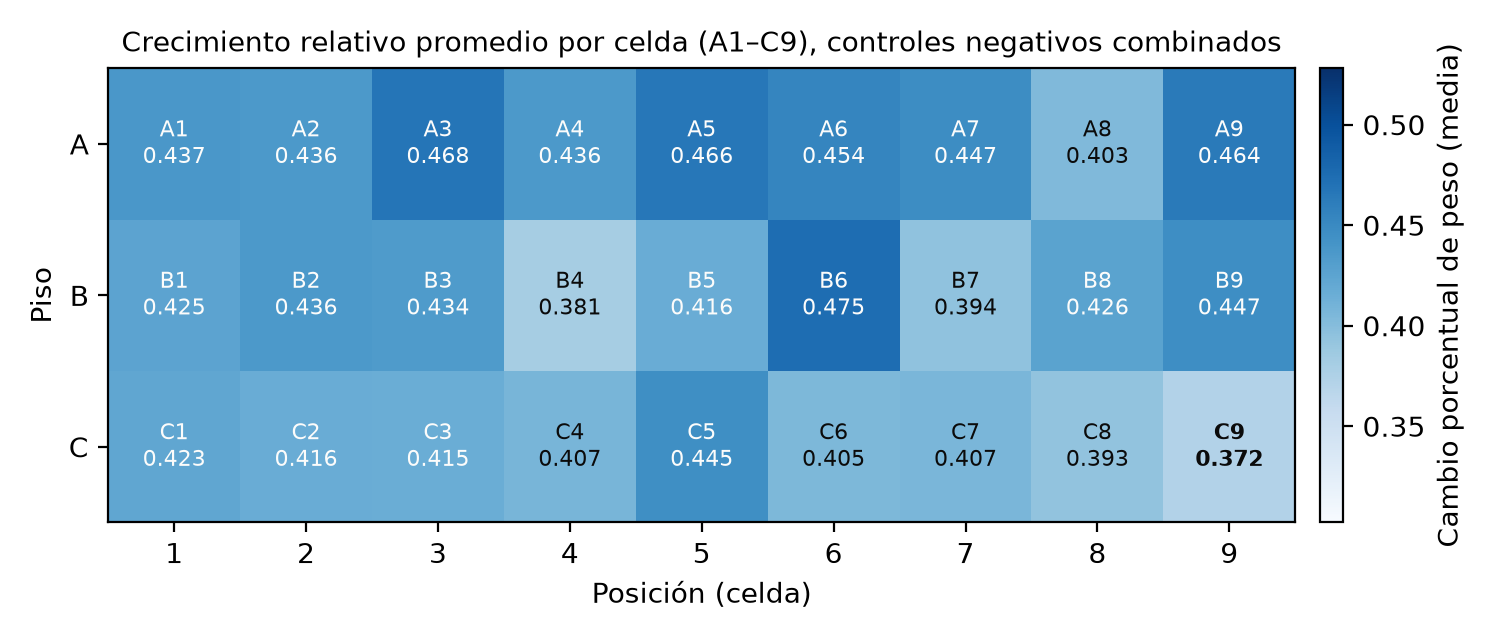
\includegraphics[width=0.85\linewidth]{datos/img/ctrl_pct_change_heatmap.png}
    \caption{Mapa de calor del crecimiento relativo promedio (cambio porcentual de peso) por celda (A1--C9) en controles negativos combinados. La celda C9 se destaca por presentar el menor valor promedio del conjunto.}
    \label{fig:ctrl_pct_change_heatmap}
\end{figure}

El análisis post-hoc por pares con corrección FDR identificó que las diferencias estuvieron principalmente asociadas a la celda C9, que presentó menor crecimiento relativo que varias celdas (Tabla~\ref{tab:ctrl_posthoc}).

\begin{table}[h]
\centering
\caption{Comparaciones post-hoc significativas (FDR) para el cambio porcentual de peso en el análisis A1--C9. Cada celda tiene \(n = 3\).}
\label{tab:ctrl_posthoc}
\begin{tabular}{lccc}
\hline
Comparación & Media celda 1 & Media celda 2 & Diferencia \\
\hline
C9 vs B8 & 0.3721 & 0.4263 & 0.0542 \\
C9 vs A1 & 0.3721 & 0.4373 & 0.0652 \\
C9 vs A9 & 0.3721 & 0.4636 & 0.0915 \\
C9 vs A3 & 0.3721 & 0.4676 & 0.0955 \\
C9 vs B6 & 0.3721 & 0.4751 & 0.1030 \\
\hline
\end{tabular}
\end{table}

Notar que si bien C9 presentó una desviación estándar muy pequeña (0.0114), esto refleja la consistencia entre las tres réplicas, no necesariamente una mayor precisión a nivel poblacional.

\begin{figure}[H]
    \centering
    \includegraphics[width=\linewidth]{datos/software_data/analysis/negative_control_combined/negative_control_combined_pct_change_tray_cell_barplot.png}
    \caption{Crecimiento relativo (cambio porcentual de peso) por celda individual (A1--C9) en controles negativos combinados. Se observa el menor crecimiento relativo de la celda C9 respecto de las demás.}
    \label{fig:ctrl_pct_change_all}
\end{figure}

\subsubsection{Conclusión parcial}

En los controles negativos combinados se detectó un efecto espacial general asociado al piso de la bandeja (A \(>\) B \(>\) C), pero no a los ejes izquierda-centro-derecha ni frente-medio-atrás. Sin embargo, al analizar cada celda individual A1--C9, se observaron diferencias significativas entre posiciones específicas. El análisis post-hoc indicó que estas diferencias estuvieron principalmente asociadas a la celda C9, que presentó menor crecimiento relativo que varias celdas de mayor crecimiento. Esto sugiere que el control negativo no fue completamente homogéneo a escala espacial fina, por lo que los análisis de tratamientos deberían considerar o controlar posibles efectos de posición.

\include{secciones/discusion}
\include{secciones/conclusiones}

\printbibliography

\begin{appendices}
\include{secciones/apendices}
\end{appendices}

\end{document}
